%!TEX TS-program = xelatex
%!TEX encoding = UTF-8 Unicode
%times,


%%%%%%%%%%%%%%%%%%%%%%%%%%%%%%%%%%%%%%%%%
% The Legrand Orange Book
% LaTeX Template
% Version 2.0 (9/2/15)
%
% This template has been downloaded from:
% http://www.LaTeXTemplates.com
% License:
% CC BY-NC-SA 3.0 (http://creativecommons.org/licenses/by-nc-sa/3.0/)
% Important note:
% Chapter heading images should have a 2:1 width:height ratio,
% e.g. 920px width and 460px height.
%%%%%%%%%%%%%%%%%%%%%%%%%%%%%%%%%%%%%%%%%

\documentclass[11pt,fleqn,twoside]{book}
\makeatletter
\usepackage{indentfirst}
\usepackage{xeCJK}
\setCJKmainfont[BoldFont={SimHei},ItalicFont={KaiTi}]{SimSun}
\usepackage{bm}
\usepackage{amssymb}
\usepackage{mathrsfs}
\usepackage{ulem}
\usepackage[version=3]{mhchem}
\usepackage{draftwatermark}
\SetWatermarkText{\textsc{Draft Translation}}
\SetWatermarkLightness{0.88}
\SetWatermarkScale{0.4}
\usepackage{setspace}
\usepackage{marginfix}
%\include{marginpar}
%%%%%%%%%%%%%%%%%%%%%%%%%%%%%%%%%%%%%%%%%
% The Legrand Orange Book
% Structural Definitions File
% Version 2.0 (9/2/15)
%
% Original author:
% Mathias Legrand (legrand.mathias@gmail.com) with modifications by:
% Vel (vel@latextemplates.com)
% 
% This file has been downloaded from:
% http://www.LaTeXTemplates.com
%
% License:
% CC BY-NC-SA 3.0 (http://creativecommons.org/licenses/by-nc-sa/3.0/)
%
%%%%%%%%%%%%%%%%%%%%%%%%%%%%%%%%%%%%%%%%%

%----------------------------------------------------------------------------------------
%	VARIOUS REQUIRED PACKAGES AND CONFIGURATIONS
%----------------------------------------------------------------------------------------

\usepackage[top=3cm,bottom=3cm,left=3cm,right=3cm,headsep=10pt,a4paper,outer=7cm,marginparwidth=4cm, marginparsep=2cm]{geometry} % Page margins

\usepackage{graphicx} % Required for including pictures
\graphicspath{{Pictures/}} % Specifies the directory where pictures are stored

\usepackage{lipsum} % Inserts dummy text

\usepackage{tikz} % Required for drawing custom shapes

\usepackage[english]{babel} % English language/hyphenation

\usepackage{enumitem} % Customize lists
\setlist{nolistsep} % Reduce spacing between bullet points and numbered lists

\usepackage{booktabs} % Required for nicer horizontal rules in tables

\usepackage{xcolor} % Required for specifying colors by name
\definecolor{ocre}{RGB}{243,102,25} % Define the orange color used for highlighting throughout the book

%----------------------------------------------------------------------------------------
%	FONTS
%----------------------------------------------------------------------------------------

\usepackage{avant} % Use the Avantgarde font for headings
%\usepackage{times} % Use the Times font for headings
%\usepackage{mathptmx} % Use the Adobe Times Roman as the default text font together with math symbols from the Sym­bol, Chancery and Com­puter Modern fonts

%\usepackage{microtype} % Slightly tweak font spacing for aesthetics
\usepackage[utf8]{inputenc} % Required for including letters with accents
\usepackage[T1]{fontenc} % Use 8-bit encoding that has 256 glyphs

%----------------------------------------------------------------------------------------
%	BIBLIOGRAPHY AND INDEX
%----------------------------------------------------------------------------------------

%\usepackage[style=alphabetic,citestyle=numeric,sorting=nyt,sortcites=true,autopunct=true,babel=hyphen,hyperref=true,abbreviate=false,backref=true,backend=biber]{biblatex}
%\addbibresource{bibliography.bib} % BibTeX bibliography file
%\defbibheading{bibempty}{}

\usepackage{calc} % For simpler calculation - used for spacing the index letter headings correctly
\usepackage{makeidx} % Required to make an index
\makeindex % Tells LaTeX to create the files required for indexing

%----------------------------------------------------------------------------------------
%	MAIN TABLE OF CONTENTS
%----------------------------------------------------------------------------------------

\usepackage{titletoc} % Required for manipulating the table of contents

\contentsmargin{0cm} % Removes the default margin

% Part text styling
\titlecontents{part}[0cm]
{\addvspace{20pt}\centering\large\bfseries}
{}
{}
{}

% Chapter text styling
\titlecontents{chapter}[1.25cm] % Indentation
{\addvspace{12pt}\large\sffamily\bfseries} % Spacing and font options for chapters
{\color{ocre!60}\contentslabel[\Large\thecontentslabel]{1.25cm}\color{ocre}} % Chapter number
{\color{ocre}}  
{\color{ocre!60}\normalsize\;\titlerule*[.5pc]{.}\;\thecontentspage} % Page number

% Section text styling
\titlecontents{section}[1.25cm] % Indentation
{\addvspace{3pt}\sffamily\bfseries} % Spacing and font options for sections
{\contentslabel[\thecontentslabel]{1.25cm}} % Section number
{}
{\hfill\color{black}\thecontentspage} % Page number
[]

% Subsection text styling
\titlecontents{subsection}[1.25cm] % Indentation
{\addvspace{1pt}\sffamily\small} % Spacing and font options for subsections
{\contentslabel[\thecontentslabel]{1.25cm}} % Subsection number
{}
{\ \titlerule*[.5pc]{.}\;\thecontentspage} % Page number
[]

% List of figures
\titlecontents{figure}[0em]
{\addvspace{-5pt}\sffamily}
{\thecontentslabel\hspace*{1em}}
{}
{\ \titlerule*[.5pc]{.}\;\thecontentspage}
[]

% List of tables
\titlecontents{table}[0em]
{\addvspace{-5pt}\sffamily}
{\thecontentslabel\hspace*{1em}}
{}
{\ \titlerule*[.5pc]{.}\;\thecontentspage}
[]

%----------------------------------------------------------------------------------------
%	MINI TABLE OF CONTENTS IN PART HEADS
%----------------------------------------------------------------------------------------

% Chapter text styling
\titlecontents{lchapter}[0em] % Indenting
{\addvspace{15pt}\large\sffamily\bfseries} % Spacing and font options for chapters
{\color{ocre}\contentslabel[\Large\thecontentslabel]{1.25cm}\color{ocre}} % Chapter number
{}  
{\color{ocre}\normalsize\sffamily\bfseries\;\titlerule*[.5pc]{.}\;\thecontentspage} % Page number

% Section text styling
\titlecontents{lsection}[0em] % Indenting
{\sffamily\small} % Spacing and font options for sections
{\contentslabel[\thecontentslabel]{1.25cm}} % Section number
{}
{}

% Subsection text styling
\titlecontents{lsubsection}[.5em] % Indentation
{\normalfont\footnotesize\sffamily} % Font settings
{}
{}
{}

%----------------------------------------------------------------------------------------
%	PAGE HEADERS
%----------------------------------------------------------------------------------------

\usepackage{fancyhdr} % Required for header and footer configuration

\pagestyle{fancy}
\renewcommand{\chaptermark}[1]{\markboth{\sffamily\normalsize\bfseries\chaptername\ \thechapter.\ #1}{}} % Chapter text font settings
\renewcommand{\sectionmark}[1]{\markright{\sffamily\normalsize\thesection\hspace{5pt}#1}{}} % Section text font settings
\fancyhf{} \fancyhead[LE,RO]{\sffamily\normalsize\thepage} % Font setting for the page number in the header
\fancyhead[LO]{\rightmark} % Print the nearest section name on the left side of odd pages
\fancyhead[RE]{\leftmark} % Print the current chapter name on the right side of even pages
\renewcommand{\headrulewidth}{0.5pt} % Width of the rule under the header
\addtolength{\headheight}{2.5pt} % Increase the spacing around the header slightly
\renewcommand{\footrulewidth}{0pt} % Removes the rule in the footer
\fancypagestyle{plain}{\fancyhead{}\renewcommand{\headrulewidth}{0pt}} % Style for when a plain pagestyle is specified

% Removes the header from odd empty pages at the end of chapters
\makeatletter
\renewcommand{\cleardoublepage}{
\clearpage\ifodd\c@page\else
\hbox{}
\vspace*{\fill}
\thispagestyle{empty}
\newpage
\fi}

%----------------------------------------------------------------------------------------
%	THEOREM STYLES
%----------------------------------------------------------------------------------------

\usepackage{amsmath,amsfonts,amssymb,amsthm} % For math equations, theorems, symbols, etc

\newcommand{\intoo}[2]{\mathopen{]}#1\,;#2\mathclose{[}}
\newcommand{\ud}{\mathop{\mathrm{{}d}}\mathopen{}}
\newcommand{\intff}[2]{\mathopen{[}#1\,;#2\mathclose{]}}
\newtheorem{notation}{Notation}[chapter]

% Boxed/framed environments
\newtheoremstyle{ocrenumbox}% % Theorem style name
{0pt}% Space above
{0pt}% Space below
{\normalfont}% % Body font
{}% Indent amount
{\small\bf\sffamily\color{ocre}}% % Theorem head font
{\;}% Punctuation after theorem head
{0.25em}% Space after theorem head
{\small\sffamily\color{ocre}\thmname{#1}\nobreakspace\thmnumber{\@ifnotempty{#1}{}\@upn{#2}}% Theorem text (e.g. Theorem 2.1)
\thmnote{\nobreakspace\the\thm@notefont\sffamily\bfseries\color{black}---\nobreakspace#3.}} % Optional theorem note
\renewcommand{\qedsymbol}{$\blacksquare$}% Optional qed square

\newtheoremstyle{blacknumex}% Theorem style name
{5pt}% Space above
{5pt}% Space below
{\normalfont}% Body font
{} % Indent amount
{\small\bf\sffamily}% Theorem head font
{\;}% Punctuation after theorem head
{0.25em}% Space after theorem head
{\small\sffamily{\tiny\ensuremath{\blacksquare}}\nobreakspace\thmname{#1}\nobreakspace\thmnumber{\@ifnotempty{#1}{}\@upn{#2}}% Theorem text (e.g. Theorem 2.1)
\thmnote{\nobreakspace\the\thm@notefont\sffamily\bfseries---\nobreakspace#3.}}% Optional theorem note

\newtheoremstyle{blacknumbox} % Theorem style name
{0pt}% Space above
{0pt}% Space below
{\normalfont}% Body font
{}% Indent amount
{\small\bf\sffamily}% Theorem head font
{\;}% Punctuation after theorem head
{0.25em}% Space after theorem head
{\small\sffamily\thmname{#1}\nobreakspace\thmnumber{\@ifnotempty{#1}{}\@upn{#2}}% Theorem text (e.g. Theorem 2.1)
\thmnote{\nobreakspace\the\thm@notefont\sffamily\bfseries---\nobreakspace#3.}}% Optional theorem note

% Non-boxed/non-framed environments
\newtheoremstyle{ocrenum}% % Theorem style name
{5pt}% Space above
{5pt}% Space below
{\normalfont}% % Body font
{}% Indent amount
{\small\bf\sffamily\color{ocre}}% % Theorem head font
{\;}% Punctuation after theorem head
{0.25em}% Space after theorem head
{\small\sffamily\color{ocre}\thmname{#1}\nobreakspace\thmnumber{\@ifnotempty{#1}{}\@upn{#2}}% Theorem text (e.g. Theorem 2.1)
\thmnote{\nobreakspace\the\thm@notefont\sffamily\bfseries\color{black}---\nobreakspace#3.}} % Optional theorem note
\renewcommand{\qedsymbol}{$\blacksquare$}% Optional qed square
\makeatother

% Defines the theorem text style for each type of theorem to one of the three styles above
\newcounter{dummy} 
\numberwithin{dummy}{section}
\theoremstyle{ocrenumbox}
\newtheorem{theoremeT}[dummy]{Theorem}
\newtheorem{problem}{Problem}[chapter]
\newtheorem{exerciseT}{Exercise}[chapter]
\theoremstyle{blacknumex}
\newtheorem{exampleT}{Example}[chapter]
\theoremstyle{blacknumbox}
\newtheorem{vocabulary}{Vocabulary}[chapter]
\newtheorem{definitionT}{Definition}[]
\newtheorem{corollaryT}[dummy]{Corollary}
\theoremstyle{ocrenum}
\newtheorem{proposition}[dummy]{Proposition}

%----------------------------------------------------------------------------------------
%	DEFINITION OF COLORED BOXES
%----------------------------------------------------------------------------------------

\RequirePackage[framemethod=default]{mdframed} % Required for creating the theorem, definition, exercise and corollary boxes

% Theorem box
\newmdenv[skipabove=7pt,
skipbelow=7pt,
backgroundcolor=black!5,
linecolor=ocre,
innerleftmargin=5pt,
innerrightmargin=5pt,
innertopmargin=5pt,
leftmargin=0cm,
rightmargin=0cm,
innerbottommargin=5pt]{tBox}

% Exercise box	  
\newmdenv[skipabove=7pt,
skipbelow=7pt,
rightline=false,
leftline=true,
topline=false,
bottomline=false,
backgroundcolor=ocre!10,
linecolor=ocre,
innerleftmargin=5pt,
innerrightmargin=5pt,
innertopmargin=5pt,
innerbottommargin=5pt,
leftmargin=0cm,
rightmargin=0cm,
linewidth=4pt]{eBox}	

% Definition box
\newmdenv[skipabove=7pt,
skipbelow=7pt,
rightline=false,
leftline=true,
topline=false,
bottomline=false,
linecolor=ocre,
innerleftmargin=5pt,
innerrightmargin=5pt,
innertopmargin=0pt,
leftmargin=0cm,
rightmargin=0cm,
linewidth=4pt,
innerbottommargin=0pt]{dBox}	

% Corollary box
\newmdenv[skipabove=7pt,
skipbelow=7pt,
rightline=false,
leftline=true,
topline=false,
bottomline=false,
linecolor=gray,
backgroundcolor=black!5,
innerleftmargin=5pt,
innerrightmargin=5pt,
innertopmargin=5pt,
leftmargin=0cm,
rightmargin=0cm,
linewidth=4pt,
innerbottommargin=5pt]{cBox}

% Creates an environment for each type of theorem and assigns it a theorem text style from the "Theorem Styles" section above and a colored box from above
\newenvironment{theorem}{\begin{tBox}\begin{theoremeT}}{\end{theoremeT}\end{tBox}}
\newenvironment{exercise}{\begin{eBox}\begin{exerciseT}}{\hfill{\color{ocre}\tiny\ensuremath{\blacksquare}}\end{exerciseT}\end{eBox}}				  
\newenvironment{definition}{\begin{dBox}\begin{definitionT}}{\end{definitionT}\end{dBox}}	
\newenvironment{example}{\begin{exampleT}}{\hfill{\tiny\ensuremath{\blacksquare}}\end{exampleT}}		
\newenvironment{corollary}{\begin{cBox}\begin{corollaryT}}{\end{corollaryT}\end{cBox}}	

%----------------------------------------------------------------------------------------
%	REMARK ENVIRONMENT
%----------------------------------------------------------------------------------------

\newenvironment{remark}{\par\vspace{10pt}\small % Vertical white space above the remark and smaller font size
\begin{list}{}{
\leftmargin=35pt % Indentation on the left
\rightmargin=25pt}\item\ignorespaces % Indentation on the right
\makebox[-2.5pt]{\begin{tikzpicture}[overlay]
\node[draw=ocre!60,line width=1pt,circle,fill=ocre!25,font=\sffamily\bfseries,inner sep=2pt,outer sep=0pt] at (-15pt,0pt){\textcolor{ocre}{R}};\end{tikzpicture}} % Orange R in a circle
\advance\baselineskip -1pt}{\end{list}\vskip5pt} % Tighter line spacing and white space after remark

%----------------------------------------------------------------------------------------
%	SECTION NUMBERING IN THE MARGIN
%----------------------------------------------------------------------------------------

\makeatletter
\renewcommand{\@seccntformat}[1]{\llap{\textcolor{ocre}{\csname the#1\endcsname}\hspace{1em}}}                    
\renewcommand{\section}{\@startsection{section}{1}{\z@}
{-4ex \@plus -1ex \@minus -.4ex}
{1ex \@plus.2ex }
{\normalfont\large\sffamily\bfseries}}
\renewcommand{\subsection}{\@startsection {subsection}{2}{\z@}
{-3ex \@plus -0.1ex \@minus -.4ex}
{0.5ex \@plus.2ex }
{\normalfont\sffamily\bfseries}}
\renewcommand{\subsubsection}{\@startsection {subsubsection}{3}{\z@}
{-2ex \@plus -0.1ex \@minus -.2ex}
{.2ex \@plus.2ex }
{\normalfont\small\sffamily\bfseries}}                        
\renewcommand\paragraph{\@startsection{paragraph}{4}{\z@}
{-2ex \@plus-.2ex \@minus .2ex}
{.1ex}
{\normalfont\small\sffamily\bfseries}}

%----------------------------------------------------------------------------------------
%	PART HEADINGS
%----------------------------------------------------------------------------------------

% numbered part in the table of contents
\newcommand{\@mypartnumtocformat}[2]{%
\setlength\fboxsep{0pt}%
\noindent\colorbox{ocre!20}{\strut\parbox[c][.7cm]{\ecart}{\color{ocre!70}\Large\sffamily\bfseries\centering#1}}\hskip\esp\colorbox{ocre!40}{\strut\parbox[c][.7cm]{\linewidth-\ecart-\esp}{\Large\sffamily\centering#2}}}%
%%%%%%%%%%%%%%%%%%%%%%%%%%%%%%%%%%
% unnumbered part in the table of contents
\newcommand{\@myparttocformat}[1]{%
\setlength\fboxsep{0pt}%
\noindent\colorbox{ocre!40}{\strut\parbox[c][.7cm]{\linewidth}{\Large\sffamily\centering#1}}}%
%%%%%%%%%%%%%%%%%%%%%%%%%%%%%%%%%%
\newlength\esp
\setlength\esp{4pt}
\newlength\ecart
\setlength\ecart{1.2cm-\esp}
\newcommand{\thepartimage}{}%
\newcommand{\partimage}[1]{\renewcommand{\thepartimage}{#1}}%
\def\@part[#1]#2{%
\ifnum \c@secnumdepth >-2\relax%
\refstepcounter{part}%
\addcontentsline{toc}{part}{\texorpdfstring{\protect\@mypartnumtocformat{\thepart}{#1}}{\partname~\thepart\ ---\ #1}}
\else%
\addcontentsline{toc}{part}{\texorpdfstring{\protect\@myparttocformat{#1}}{#1}}%
\fi%
\startcontents%
\markboth{}{}%
{\thispagestyle{empty}%
\begin{tikzpicture}[remember picture,overlay]%
\node at (current page.north west){\begin{tikzpicture}[remember picture,overlay]%	
\fill[ocre!20](0cm,0cm) rectangle (\paperwidth,-\paperheight);
\node[anchor=north] at (4cm,-3.25cm){\color{ocre!40}\fontsize{220}{100}\sffamily\bfseries\@Roman\c@part}; 
\node[anchor=south east] at (\paperwidth-1cm,-\paperheight+1cm){\parbox[t][][t]{8.5cm}{
\printcontents{l}{0}{\setcounter{tocdepth}{1}}%
}};
\node[anchor=north east] at (\paperwidth-1.5cm,-3.25cm){\parbox[t][][t]{15cm}{\strut\raggedleft\color{white}\fontsize{30}{30}\sffamily\bfseries#2}};
\end{tikzpicture}};
\end{tikzpicture}}%
\@endpart}
\def\@spart#1{%
\startcontents%
\phantomsection
{\thispagestyle{empty}%
\begin{tikzpicture}[remember picture,overlay]%
\node at (current page.north west){\begin{tikzpicture}[remember picture,overlay]%	
\fill[ocre!20](0cm,0cm) rectangle (\paperwidth,-\paperheight);
\node[anchor=north east] at (\paperwidth-1.5cm,-3.25cm){\parbox[t][][t]{15cm}{\strut\raggedleft\color{white}\fontsize{30}{30}\sffamily\bfseries#1}};
\end{tikzpicture}};
\end{tikzpicture}}
\addcontentsline{toc}{part}{\texorpdfstring{%
\setlength\fboxsep{0pt}%
\noindent\protect\colorbox{ocre!40}{\strut\protect\parbox[c][.7cm]{\linewidth}{\Large\sffamily\protect\centering #1\quad\mbox{}}}}{#1}}%
\@endpart}
\def\@endpart{\vfil\newpage
\if@twoside
\if@openright
\null
\thispagestyle{empty}%
\newpage
\fi
\fi
\if@tempswa
\twocolumn
\fi}

%----------------------------------------------------------------------------------------
%	CHAPTER HEADINGS
%----------------------------------------------------------------------------------------

\newcommand{\thechapterimage}{}%
\newcommand{\chapterimage}[1]{\renewcommand{\thechapterimage}{#1}}%
\def\@makechapterhead#1{%
{\parindent \z@ \raggedright \normalfont
\ifnum \c@secnumdepth >\m@ne
\if@mainmatter
\begin{tikzpicture}[remember picture,overlay]
\node at (current page.north west)
{\begin{tikzpicture}[remember picture,overlay]
\node[anchor=north west,inner sep=0pt] at (0,0) {\includegraphics[width=\paperwidth]{\thechapterimage}};
\draw[anchor=west] (\Gm@lmargin,-9cm) node [line width=2pt,rounded corners=15pt,draw=ocre,fill=white,fill opacity=0.5,inner sep=15pt]{\strut\makebox[22cm]{}};
\draw[anchor=west] (\Gm@lmargin+.3cm,-9cm) node {\huge\sffamily\bfseries\color{black}\thechapter. #1\strut};
\end{tikzpicture}};
\end{tikzpicture}
\else
\begin{tikzpicture}[remember picture,overlay]
\node at (current page.north west)
{\begin{tikzpicture}[remember picture,overlay]
\node[anchor=north west,inner sep=0pt] at (0,0) {\includegraphics[width=\paperwidth]{\thechapterimage}};
\draw[anchor=west] (\Gm@lmargin,-9cm) node [line width=2pt,rounded corners=15pt,draw=ocre,fill=white,fill opacity=0.5,inner sep=15pt]{\strut\makebox[22cm]{}};
\draw[anchor=west] (\Gm@lmargin+.3cm,-9cm) node {\huge\sffamily\bfseries\color{black}#1\strut};
\end{tikzpicture}};
\end{tikzpicture}
\fi\fi\par\vspace*{270\p@}}}

%-------------------------------------------

\def\@makeschapterhead#1{%
\begin{tikzpicture}[remember picture,overlay]
\node at (current page.north west)
{\begin{tikzpicture}[remember picture,overlay]
\node[anchor=north west,inner sep=0pt] at (0,0) {\includegraphics[width=\paperwidth]{\thechapterimage}};
\draw[anchor=west] (\Gm@lmargin,-9cm) node [line width=2pt,rounded corners=15pt,draw=ocre,fill=white,fill opacity=0.5,inner sep=15pt]{\strut\makebox[22cm]{}};
\draw[anchor=west] (\Gm@lmargin+.3cm,-9cm) node {\huge\sffamily\bfseries\color{black}#1\strut};
\end{tikzpicture}};
\end{tikzpicture}
\par\vspace*{270\p@}}
\makeatother

%----------------------------------------------------------------------------------------
%	HYPERLINKS IN THE DOCUMENTS
%----------------------------------------------------------------------------------------

\usepackage[colorlinks,linkcolor=red,anchorcolor=blue,citecolor=blue,urlcolor=black]{hyperref}
\hypersetup{hidelinks,backref=true,pagebackref=true,hyperindex=true,colorlinks=true,breaklinks=true,urlcolor= ocre,bookmarks=true,bookmarksopen=false,pdftitle={Title},pdfauthor={Author}}
\usepackage{bookmark}
\bookmarksetup{
open,
numbered,
addtohook={%
\ifnum\bookmarkget{level}=0 % chapter
\bookmarksetup{bold}%
\fi
\ifnum\bookmarkget{level}=-1 % part
\bookmarksetup{color=ocre,bold}%
\fi
}
} 
\usepackage{xypic}
\def\UrlBreaks{\do\A\do\B\do\C\do\D\do\E\do\F\do\G\do\H\do\I\do\J
\do\K\do\L\do\M\do\N\do\O\do\P\do\Q\do\R\do\S\do\T\do\U\do\V
\do\W\do\X\do\Y\do\Z\do\[\do\\\do\]\do\^\do\_\do\`\do\a\do\b
\do\c\do\d\do\e\do\f\do\g\do\h\do\i\do\j\do\k\do\l\do\m\do\n
\do\o\do\p\do\q\do\r\do\s\do\t\do\u\do\v\do\w\do\x\do\y\do\z
\do\.\do\@\do\\\do\/\do\!\do\_\do\|\do\;\do\>\do\]\do\)\do\,
\do\?\do\'\do+\do\=\do\#} 


\newcounter{mparcnt}
\renewcommand\themparcnt{\small{$^{\arabic{mparcnt}}$}}
\newcommand\mpar[1]{\refstepcounter{mparcnt}{$^{\arabic{mparcnt}}$}\marginpar{\themparcnt\scriptsize#1}}
\makeatother



%\makeatletter
%\def\mpar#1{%
%  {\refstepcounter{mparcnt}{$^{\arabic{mparcnt}}$}\marginpar{\themparcnt\tiny#1}}%
%}
%\def\mpar@macro#1[#2]{%
%  {\refstepcounter{mparcnt}{$^{\arabic{mparcnt}}$}\marginnote[#2]{\themparcnt\tiny#1}}
%}
%\makeatother

\begin{document}

%\pagestyle{fancy}

%----------------------------------------------------------------------------------------
%	TITLE PAGE
%----------------------------------------------------------------------------------------

\begingroup
\thispagestyle{empty}
\begin{tikzpicture}[remember picture,overlay]
\coordinate [below=12cm] (midpoint) at (current page.north);
\node at (current page.north west)
{\begin{tikzpicture}[remember picture,overlay]
\node[anchor=north west,inner sep=0pt] at (0,0) {
\includegraphics[width=\paperwidth]{background}}; % Background image
\draw[anchor=north] (midpoint) node [fill=ocre!30!white,fill opacity=0.6,text opacity=1,inner sep=1cm]{\Huge\centering\bfseries\sffamily\parbox[c][][t]{\paperwidth}{\centering Physics from Symmetry \\[15pt] % Book title
{\Large $1^{st}$ edition}\\[20pt] % Subtitle
{\huge } % Author name
{\huge Translate Version: \chntoday}
}};
\end{tikzpicture}};
\end{tikzpicture}
\vfill
\endgroup

%----------------------------------------------------------------------------------------
%	COPYRIGHT PAGE
%----------------------------------------------------------------------------------------

\newpage
~\vfill
\thispagestyle{empty}

\noindent Copyright \copyright\ 2016 Chaoli-Translating-Group \\ % Copyright notice

\noindent \textsc{Published by Non}\\ % Publisher

\noindent \textsc{https://github.com/laserroger/Physics-from-Symmetry/}\\ % URL

\noindent Licensed under the Creative Commons Attribution-NonCommercial 3.0 Unported License (the ``License''). You may not use this file except in compliance with the License. You may obtain a copy of the License at \url{http://creativecommons.org/licenses/by-nc/3.0}. Unless required by applicable law or agreed to in writing, software distributed under the License is distributed on an \textsc{``as is'' basis, without warranties or conditions of any kind}, either express or implied. See the License for the specific language governing permissions and limitations under the License.\\ % License information

%\noindent \textit{First printing, March 2013} % Printing/edition date

%----------------------------------------------------------------------------------------
%	TABLE OF CONTENTS
%----------------------------------------------------------------------------------------
\begin{spacing}{1.4}
\chapterimage{chapter_head_1.pdf} % Chapter heading image


\pagestyle{empty} % No headers


\cleardoublepage % Forces the first chapter to start on an odd page so it's on the right

\pagestyle{fancy} % Print headers again

%----------------------------------------------------------------------------------------
%	PART
%----------------------------------------------------------------------------------------

%\part*{Preface}
%!TEX TS-program = xelatex
%!TEX encoding = UTF-8 Unicode
%times,


%%%%%%%%%%%%%%%%%%%%%%%%%%%%%%%%%%%%%%%%%
% The Legrand Orange Book
% LaTeX Template
% Version 2.0 (9/2/15)
%
% This template has been downloaded from:
% http://www.LaTeXTemplates.com
% License:
% CC BY-NC-SA 3.0 (http://creativecommons.org/licenses/by-nc-sa/3.0/)
% Important note:
% Chapter heading images should have a 2:1 width:height ratio,
% e.g. 920px width and 460px height.
%%%%%%%%%%%%%%%%%%%%%%%%%%%%%%%%%%%%%%%%%

\documentclass[11pt,fleqn]{book}
\usepackage{xeCJK}
\setCJKmainfont[BoldFont={STHeiti},ItalicFont=STKaiti]{STSong}
\usepackage{bm}
\usepackage{amssymb}
\usepackage{mathrsfs}
\usepackage[version=3]{mhchem}
\usepackage{draftwatermark}
\SetWatermarkText{\textsc{Draft Translation}}
\SetWatermarkLightness{0.88}
\SetWatermarkScale{0.4}


%%%%%%%%%%%%%%%%%%%%%%%%%%%%%%%%%%%%%%%%%
% The Legrand Orange Book
% Structural Definitions File
% Version 2.0 (9/2/15)
%
% Original author:
% Mathias Legrand (legrand.mathias@gmail.com) with modifications by:
% Vel (vel@latextemplates.com)
% 
% This file has been downloaded from:
% http://www.LaTeXTemplates.com
%
% License:
% CC BY-NC-SA 3.0 (http://creativecommons.org/licenses/by-nc-sa/3.0/)
%
%%%%%%%%%%%%%%%%%%%%%%%%%%%%%%%%%%%%%%%%%

%----------------------------------------------------------------------------------------
%	VARIOUS REQUIRED PACKAGES AND CONFIGURATIONS
%----------------------------------------------------------------------------------------

\usepackage[top=3cm,bottom=3cm,left=3cm,right=3cm,headsep=10pt,a4paper,outer=7cm,marginparwidth=4cm, marginparsep=2cm]{geometry} % Page margins

\usepackage{graphicx} % Required for including pictures
\graphicspath{{Pictures/}} % Specifies the directory where pictures are stored

\usepackage{lipsum} % Inserts dummy text

\usepackage{tikz} % Required for drawing custom shapes

\usepackage[english]{babel} % English language/hyphenation

\usepackage{enumitem} % Customize lists
\setlist{nolistsep} % Reduce spacing between bullet points and numbered lists

\usepackage{booktabs} % Required for nicer horizontal rules in tables

\usepackage{xcolor} % Required for specifying colors by name
\definecolor{ocre}{RGB}{243,102,25} % Define the orange color used for highlighting throughout the book

%----------------------------------------------------------------------------------------
%	FONTS
%----------------------------------------------------------------------------------------

\usepackage{avant} % Use the Avantgarde font for headings
%\usepackage{times} % Use the Times font for headings
%\usepackage{mathptmx} % Use the Adobe Times Roman as the default text font together with math symbols from the Sym­bol, Chancery and Com­puter Modern fonts

%\usepackage{microtype} % Slightly tweak font spacing for aesthetics
\usepackage[utf8]{inputenc} % Required for including letters with accents
\usepackage[T1]{fontenc} % Use 8-bit encoding that has 256 glyphs

%----------------------------------------------------------------------------------------
%	BIBLIOGRAPHY AND INDEX
%----------------------------------------------------------------------------------------

%\usepackage[style=alphabetic,citestyle=numeric,sorting=nyt,sortcites=true,autopunct=true,babel=hyphen,hyperref=true,abbreviate=false,backref=true,backend=biber]{biblatex}
%\addbibresource{bibliography.bib} % BibTeX bibliography file
%\defbibheading{bibempty}{}

\usepackage{calc} % For simpler calculation - used for spacing the index letter headings correctly
\usepackage{makeidx} % Required to make an index
\makeindex % Tells LaTeX to create the files required for indexing

%----------------------------------------------------------------------------------------
%	MAIN TABLE OF CONTENTS
%----------------------------------------------------------------------------------------

\usepackage{titletoc} % Required for manipulating the table of contents

\contentsmargin{0cm} % Removes the default margin

% Part text styling
\titlecontents{part}[0cm]
{\addvspace{20pt}\centering\large\bfseries}
{}
{}
{}

% Chapter text styling
\titlecontents{chapter}[1.25cm] % Indentation
{\addvspace{12pt}\large\sffamily\bfseries} % Spacing and font options for chapters
{\color{ocre!60}\contentslabel[\Large\thecontentslabel]{1.25cm}\color{ocre}} % Chapter number
{\color{ocre}}  
{\color{ocre!60}\normalsize\;\titlerule*[.5pc]{.}\;\thecontentspage} % Page number

% Section text styling
\titlecontents{section}[1.25cm] % Indentation
{\addvspace{3pt}\sffamily\bfseries} % Spacing and font options for sections
{\contentslabel[\thecontentslabel]{1.25cm}} % Section number
{}
{\hfill\color{black}\thecontentspage} % Page number
[]

% Subsection text styling
\titlecontents{subsection}[1.25cm] % Indentation
{\addvspace{1pt}\sffamily\small} % Spacing and font options for subsections
{\contentslabel[\thecontentslabel]{1.25cm}} % Subsection number
{}
{\ \titlerule*[.5pc]{.}\;\thecontentspage} % Page number
[]

% List of figures
\titlecontents{figure}[0em]
{\addvspace{-5pt}\sffamily}
{\thecontentslabel\hspace*{1em}}
{}
{\ \titlerule*[.5pc]{.}\;\thecontentspage}
[]

% List of tables
\titlecontents{table}[0em]
{\addvspace{-5pt}\sffamily}
{\thecontentslabel\hspace*{1em}}
{}
{\ \titlerule*[.5pc]{.}\;\thecontentspage}
[]

%----------------------------------------------------------------------------------------
%	MINI TABLE OF CONTENTS IN PART HEADS
%----------------------------------------------------------------------------------------

% Chapter text styling
\titlecontents{lchapter}[0em] % Indenting
{\addvspace{15pt}\large\sffamily\bfseries} % Spacing and font options for chapters
{\color{ocre}\contentslabel[\Large\thecontentslabel]{1.25cm}\color{ocre}} % Chapter number
{}  
{\color{ocre}\normalsize\sffamily\bfseries\;\titlerule*[.5pc]{.}\;\thecontentspage} % Page number

% Section text styling
\titlecontents{lsection}[0em] % Indenting
{\sffamily\small} % Spacing and font options for sections
{\contentslabel[\thecontentslabel]{1.25cm}} % Section number
{}
{}

% Subsection text styling
\titlecontents{lsubsection}[.5em] % Indentation
{\normalfont\footnotesize\sffamily} % Font settings
{}
{}
{}

%----------------------------------------------------------------------------------------
%	PAGE HEADERS
%----------------------------------------------------------------------------------------

\usepackage{fancyhdr} % Required for header and footer configuration

\pagestyle{fancy}
\renewcommand{\chaptermark}[1]{\markboth{\sffamily\normalsize\bfseries\chaptername\ \thechapter.\ #1}{}} % Chapter text font settings
\renewcommand{\sectionmark}[1]{\markright{\sffamily\normalsize\thesection\hspace{5pt}#1}{}} % Section text font settings
\fancyhf{} \fancyhead[LE,RO]{\sffamily\normalsize\thepage} % Font setting for the page number in the header
\fancyhead[LO]{\rightmark} % Print the nearest section name on the left side of odd pages
\fancyhead[RE]{\leftmark} % Print the current chapter name on the right side of even pages
\renewcommand{\headrulewidth}{0.5pt} % Width of the rule under the header
\addtolength{\headheight}{2.5pt} % Increase the spacing around the header slightly
\renewcommand{\footrulewidth}{0pt} % Removes the rule in the footer
\fancypagestyle{plain}{\fancyhead{}\renewcommand{\headrulewidth}{0pt}} % Style for when a plain pagestyle is specified

% Removes the header from odd empty pages at the end of chapters
\makeatletter
\renewcommand{\cleardoublepage}{
\clearpage\ifodd\c@page\else
\hbox{}
\vspace*{\fill}
\thispagestyle{empty}
\newpage
\fi}

%----------------------------------------------------------------------------------------
%	THEOREM STYLES
%----------------------------------------------------------------------------------------

\usepackage{amsmath,amsfonts,amssymb,amsthm} % For math equations, theorems, symbols, etc

\newcommand{\intoo}[2]{\mathopen{]}#1\,;#2\mathclose{[}}
\newcommand{\ud}{\mathop{\mathrm{{}d}}\mathopen{}}
\newcommand{\intff}[2]{\mathopen{[}#1\,;#2\mathclose{]}}
\newtheorem{notation}{Notation}[chapter]

% Boxed/framed environments
\newtheoremstyle{ocrenumbox}% % Theorem style name
{0pt}% Space above
{0pt}% Space below
{\normalfont}% % Body font
{}% Indent amount
{\small\bf\sffamily\color{ocre}}% % Theorem head font
{\;}% Punctuation after theorem head
{0.25em}% Space after theorem head
{\small\sffamily\color{ocre}\thmname{#1}\nobreakspace\thmnumber{\@ifnotempty{#1}{}\@upn{#2}}% Theorem text (e.g. Theorem 2.1)
\thmnote{\nobreakspace\the\thm@notefont\sffamily\bfseries\color{black}---\nobreakspace#3.}} % Optional theorem note
\renewcommand{\qedsymbol}{$\blacksquare$}% Optional qed square

\newtheoremstyle{blacknumex}% Theorem style name
{5pt}% Space above
{5pt}% Space below
{\normalfont}% Body font
{} % Indent amount
{\small\bf\sffamily}% Theorem head font
{\;}% Punctuation after theorem head
{0.25em}% Space after theorem head
{\small\sffamily{\tiny\ensuremath{\blacksquare}}\nobreakspace\thmname{#1}\nobreakspace\thmnumber{\@ifnotempty{#1}{}\@upn{#2}}% Theorem text (e.g. Theorem 2.1)
\thmnote{\nobreakspace\the\thm@notefont\sffamily\bfseries---\nobreakspace#3.}}% Optional theorem note

\newtheoremstyle{blacknumbox} % Theorem style name
{0pt}% Space above
{0pt}% Space below
{\normalfont}% Body font
{}% Indent amount
{\small\bf\sffamily}% Theorem head font
{\;}% Punctuation after theorem head
{0.25em}% Space after theorem head
{\small\sffamily\thmname{#1}\nobreakspace\thmnumber{\@ifnotempty{#1}{}\@upn{#2}}% Theorem text (e.g. Theorem 2.1)
\thmnote{\nobreakspace\the\thm@notefont\sffamily\bfseries---\nobreakspace#3.}}% Optional theorem note

% Non-boxed/non-framed environments
\newtheoremstyle{ocrenum}% % Theorem style name
{5pt}% Space above
{5pt}% Space below
{\normalfont}% % Body font
{}% Indent amount
{\small\bf\sffamily\color{ocre}}% % Theorem head font
{\;}% Punctuation after theorem head
{0.25em}% Space after theorem head
{\small\sffamily\color{ocre}\thmname{#1}\nobreakspace\thmnumber{\@ifnotempty{#1}{}\@upn{#2}}% Theorem text (e.g. Theorem 2.1)
\thmnote{\nobreakspace\the\thm@notefont\sffamily\bfseries\color{black}---\nobreakspace#3.}} % Optional theorem note
\renewcommand{\qedsymbol}{$\blacksquare$}% Optional qed square
\makeatother

% Defines the theorem text style for each type of theorem to one of the three styles above
\newcounter{dummy} 
\numberwithin{dummy}{section}
\theoremstyle{ocrenumbox}
\newtheorem{theoremeT}[dummy]{Theorem}
\newtheorem{problem}{Problem}[chapter]
\newtheorem{exerciseT}{Exercise}[chapter]
\theoremstyle{blacknumex}
\newtheorem{exampleT}{Example}[chapter]
\theoremstyle{blacknumbox}
\newtheorem{vocabulary}{Vocabulary}[chapter]
\newtheorem{definitionT}{Definition}[]
\newtheorem{corollaryT}[dummy]{Corollary}
\theoremstyle{ocrenum}
\newtheorem{proposition}[dummy]{Proposition}

%----------------------------------------------------------------------------------------
%	DEFINITION OF COLORED BOXES
%----------------------------------------------------------------------------------------

\RequirePackage[framemethod=default]{mdframed} % Required for creating the theorem, definition, exercise and corollary boxes

% Theorem box
\newmdenv[skipabove=7pt,
skipbelow=7pt,
backgroundcolor=black!5,
linecolor=ocre,
innerleftmargin=5pt,
innerrightmargin=5pt,
innertopmargin=5pt,
leftmargin=0cm,
rightmargin=0cm,
innerbottommargin=5pt]{tBox}

% Exercise box	  
\newmdenv[skipabove=7pt,
skipbelow=7pt,
rightline=false,
leftline=true,
topline=false,
bottomline=false,
backgroundcolor=ocre!10,
linecolor=ocre,
innerleftmargin=5pt,
innerrightmargin=5pt,
innertopmargin=5pt,
innerbottommargin=5pt,
leftmargin=0cm,
rightmargin=0cm,
linewidth=4pt]{eBox}	

% Definition box
\newmdenv[skipabove=7pt,
skipbelow=7pt,
rightline=false,
leftline=true,
topline=false,
bottomline=false,
linecolor=ocre,
innerleftmargin=5pt,
innerrightmargin=5pt,
innertopmargin=0pt,
leftmargin=0cm,
rightmargin=0cm,
linewidth=4pt,
innerbottommargin=0pt]{dBox}	

% Corollary box
\newmdenv[skipabove=7pt,
skipbelow=7pt,
rightline=false,
leftline=true,
topline=false,
bottomline=false,
linecolor=gray,
backgroundcolor=black!5,
innerleftmargin=5pt,
innerrightmargin=5pt,
innertopmargin=5pt,
leftmargin=0cm,
rightmargin=0cm,
linewidth=4pt,
innerbottommargin=5pt]{cBox}

% Creates an environment for each type of theorem and assigns it a theorem text style from the "Theorem Styles" section above and a colored box from above
\newenvironment{theorem}{\begin{tBox}\begin{theoremeT}}{\end{theoremeT}\end{tBox}}
\newenvironment{exercise}{\begin{eBox}\begin{exerciseT}}{\hfill{\color{ocre}\tiny\ensuremath{\blacksquare}}\end{exerciseT}\end{eBox}}				  
\newenvironment{definition}{\begin{dBox}\begin{definitionT}}{\end{definitionT}\end{dBox}}	
\newenvironment{example}{\begin{exampleT}}{\hfill{\tiny\ensuremath{\blacksquare}}\end{exampleT}}		
\newenvironment{corollary}{\begin{cBox}\begin{corollaryT}}{\end{corollaryT}\end{cBox}}	

%----------------------------------------------------------------------------------------
%	REMARK ENVIRONMENT
%----------------------------------------------------------------------------------------

\newenvironment{remark}{\par\vspace{10pt}\small % Vertical white space above the remark and smaller font size
\begin{list}{}{
\leftmargin=35pt % Indentation on the left
\rightmargin=25pt}\item\ignorespaces % Indentation on the right
\makebox[-2.5pt]{\begin{tikzpicture}[overlay]
\node[draw=ocre!60,line width=1pt,circle,fill=ocre!25,font=\sffamily\bfseries,inner sep=2pt,outer sep=0pt] at (-15pt,0pt){\textcolor{ocre}{R}};\end{tikzpicture}} % Orange R in a circle
\advance\baselineskip -1pt}{\end{list}\vskip5pt} % Tighter line spacing and white space after remark

%----------------------------------------------------------------------------------------
%	SECTION NUMBERING IN THE MARGIN
%----------------------------------------------------------------------------------------

\makeatletter
\renewcommand{\@seccntformat}[1]{\llap{\textcolor{ocre}{\csname the#1\endcsname}\hspace{1em}}}                    
\renewcommand{\section}{\@startsection{section}{1}{\z@}
{-4ex \@plus -1ex \@minus -.4ex}
{1ex \@plus.2ex }
{\normalfont\large\sffamily\bfseries}}
\renewcommand{\subsection}{\@startsection {subsection}{2}{\z@}
{-3ex \@plus -0.1ex \@minus -.4ex}
{0.5ex \@plus.2ex }
{\normalfont\sffamily\bfseries}}
\renewcommand{\subsubsection}{\@startsection {subsubsection}{3}{\z@}
{-2ex \@plus -0.1ex \@minus -.2ex}
{.2ex \@plus.2ex }
{\normalfont\small\sffamily\bfseries}}                        
\renewcommand\paragraph{\@startsection{paragraph}{4}{\z@}
{-2ex \@plus-.2ex \@minus .2ex}
{.1ex}
{\normalfont\small\sffamily\bfseries}}

%----------------------------------------------------------------------------------------
%	PART HEADINGS
%----------------------------------------------------------------------------------------

% numbered part in the table of contents
\newcommand{\@mypartnumtocformat}[2]{%
\setlength\fboxsep{0pt}%
\noindent\colorbox{ocre!20}{\strut\parbox[c][.7cm]{\ecart}{\color{ocre!70}\Large\sffamily\bfseries\centering#1}}\hskip\esp\colorbox{ocre!40}{\strut\parbox[c][.7cm]{\linewidth-\ecart-\esp}{\Large\sffamily\centering#2}}}%
%%%%%%%%%%%%%%%%%%%%%%%%%%%%%%%%%%
% unnumbered part in the table of contents
\newcommand{\@myparttocformat}[1]{%
\setlength\fboxsep{0pt}%
\noindent\colorbox{ocre!40}{\strut\parbox[c][.7cm]{\linewidth}{\Large\sffamily\centering#1}}}%
%%%%%%%%%%%%%%%%%%%%%%%%%%%%%%%%%%
\newlength\esp
\setlength\esp{4pt}
\newlength\ecart
\setlength\ecart{1.2cm-\esp}
\newcommand{\thepartimage}{}%
\newcommand{\partimage}[1]{\renewcommand{\thepartimage}{#1}}%
\def\@part[#1]#2{%
\ifnum \c@secnumdepth >-2\relax%
\refstepcounter{part}%
\addcontentsline{toc}{part}{\texorpdfstring{\protect\@mypartnumtocformat{\thepart}{#1}}{\partname~\thepart\ ---\ #1}}
\else%
\addcontentsline{toc}{part}{\texorpdfstring{\protect\@myparttocformat{#1}}{#1}}%
\fi%
\startcontents%
\markboth{}{}%
{\thispagestyle{empty}%
\begin{tikzpicture}[remember picture,overlay]%
\node at (current page.north west){\begin{tikzpicture}[remember picture,overlay]%	
\fill[ocre!20](0cm,0cm) rectangle (\paperwidth,-\paperheight);
\node[anchor=north] at (4cm,-3.25cm){\color{ocre!40}\fontsize{220}{100}\sffamily\bfseries\@Roman\c@part}; 
\node[anchor=south east] at (\paperwidth-1cm,-\paperheight+1cm){\parbox[t][][t]{8.5cm}{
\printcontents{l}{0}{\setcounter{tocdepth}{1}}%
}};
\node[anchor=north east] at (\paperwidth-1.5cm,-3.25cm){\parbox[t][][t]{15cm}{\strut\raggedleft\color{white}\fontsize{30}{30}\sffamily\bfseries#2}};
\end{tikzpicture}};
\end{tikzpicture}}%
\@endpart}
\def\@spart#1{%
\startcontents%
\phantomsection
{\thispagestyle{empty}%
\begin{tikzpicture}[remember picture,overlay]%
\node at (current page.north west){\begin{tikzpicture}[remember picture,overlay]%	
\fill[ocre!20](0cm,0cm) rectangle (\paperwidth,-\paperheight);
\node[anchor=north east] at (\paperwidth-1.5cm,-3.25cm){\parbox[t][][t]{15cm}{\strut\raggedleft\color{white}\fontsize{30}{30}\sffamily\bfseries#1}};
\end{tikzpicture}};
\end{tikzpicture}}
\addcontentsline{toc}{part}{\texorpdfstring{%
\setlength\fboxsep{0pt}%
\noindent\protect\colorbox{ocre!40}{\strut\protect\parbox[c][.7cm]{\linewidth}{\Large\sffamily\protect\centering #1\quad\mbox{}}}}{#1}}%
\@endpart}
\def\@endpart{\vfil\newpage
\if@twoside
\if@openright
\null
\thispagestyle{empty}%
\newpage
\fi
\fi
\if@tempswa
\twocolumn
\fi}

%----------------------------------------------------------------------------------------
%	CHAPTER HEADINGS
%----------------------------------------------------------------------------------------

\newcommand{\thechapterimage}{}%
\newcommand{\chapterimage}[1]{\renewcommand{\thechapterimage}{#1}}%
\def\@makechapterhead#1{%
{\parindent \z@ \raggedright \normalfont
\ifnum \c@secnumdepth >\m@ne
\if@mainmatter
\begin{tikzpicture}[remember picture,overlay]
\node at (current page.north west)
{\begin{tikzpicture}[remember picture,overlay]
\node[anchor=north west,inner sep=0pt] at (0,0) {\includegraphics[width=\paperwidth]{\thechapterimage}};
\draw[anchor=west] (\Gm@lmargin,-9cm) node [line width=2pt,rounded corners=15pt,draw=ocre,fill=white,fill opacity=0.5,inner sep=15pt]{\strut\makebox[22cm]{}};
\draw[anchor=west] (\Gm@lmargin+.3cm,-9cm) node {\huge\sffamily\bfseries\color{black}\thechapter. #1\strut};
\end{tikzpicture}};
\end{tikzpicture}
\else
\begin{tikzpicture}[remember picture,overlay]
\node at (current page.north west)
{\begin{tikzpicture}[remember picture,overlay]
\node[anchor=north west,inner sep=0pt] at (0,0) {\includegraphics[width=\paperwidth]{\thechapterimage}};
\draw[anchor=west] (\Gm@lmargin,-9cm) node [line width=2pt,rounded corners=15pt,draw=ocre,fill=white,fill opacity=0.5,inner sep=15pt]{\strut\makebox[22cm]{}};
\draw[anchor=west] (\Gm@lmargin+.3cm,-9cm) node {\huge\sffamily\bfseries\color{black}#1\strut};
\end{tikzpicture}};
\end{tikzpicture}
\fi\fi\par\vspace*{270\p@}}}

%-------------------------------------------

\def\@makeschapterhead#1{%
\begin{tikzpicture}[remember picture,overlay]
\node at (current page.north west)
{\begin{tikzpicture}[remember picture,overlay]
\node[anchor=north west,inner sep=0pt] at (0,0) {\includegraphics[width=\paperwidth]{\thechapterimage}};
\draw[anchor=west] (\Gm@lmargin,-9cm) node [line width=2pt,rounded corners=15pt,draw=ocre,fill=white,fill opacity=0.5,inner sep=15pt]{\strut\makebox[22cm]{}};
\draw[anchor=west] (\Gm@lmargin+.3cm,-9cm) node {\huge\sffamily\bfseries\color{black}#1\strut};
\end{tikzpicture}};
\end{tikzpicture}
\par\vspace*{270\p@}}
\makeatother

%----------------------------------------------------------------------------------------
%	HYPERLINKS IN THE DOCUMENTS
%----------------------------------------------------------------------------------------

\usepackage[colorlinks,linkcolor=red,anchorcolor=blue,citecolor=blue,urlcolor=black]{hyperref}
\hypersetup{hidelinks,backref=true,pagebackref=true,hyperindex=true,colorlinks=true,breaklinks=true,urlcolor= ocre,bookmarks=true,bookmarksopen=false,pdftitle={Title},pdfauthor={Author}}
\usepackage{bookmark}
\bookmarksetup{
open,
numbered,
addtohook={%
\ifnum\bookmarkget{level}=0 % chapter
\bookmarksetup{bold}%
\fi
\ifnum\bookmarkget{level}=-1 % part
\bookmarksetup{color=ocre,bold}%
\fi
}
} 
\usepackage{xypic}

\begin{document}

%\pagestyle{fancy}

%----------------------------------------------------------------------------------------
%	TITLE PAGE
%----------------------------------------------------------------------------------------

\begingroup
\thispagestyle{empty}
\begin{tikzpicture}[remember picture,overlay]
\coordinate [below=12cm] (midpoint) at (current page.north);
\node at (current page.north west)
{\begin{tikzpicture}[remember picture,overlay]
\node[anchor=north west,inner sep=0pt] at (0,0) {
\includegraphics[width=\paperwidth]{background}}; % Background image
\draw[anchor=north] (midpoint) node [fill=ocre!30!white,fill opacity=0.6,text opacity=1,inner sep=1cm]{\Huge\centering\bfseries\sffamily\parbox[c][][t]{\paperwidth}{\centering Physics from Symmetry. \\[15pt] % Book title
{\Large $1^{st}$ edition}\\[20pt] % Subtitle
{\huge }}}; % Author name
\end{tikzpicture}};
\end{tikzpicture}
\vfill
\endgroup

%----------------------------------------------------------------------------------------
%	COPYRIGHT PAGE
%----------------------------------------------------------------------------------------

\newpage
~\vfill
\thispagestyle{empty}

\noindent Copyright \copyright\ 2016 balabala \\ % Copyright notice

\noindent \textsc{Published by Non}\\ % Publisher

\noindent \textsc{https://github.com/laserroger/Physics-from-Symmetry/}\\ % URL

\noindent Licensed under the Creative Commons Attribution-NonCommercial 3.0 Unported License (the ``License''). You may not use this file except in compliance with the License. You may obtain a copy of the License at \url{http://creativecommons.org/licenses/by-nc/3.0}. Unless required by applicable law or agreed to in writing, software distributed under the License is distributed on an \textsc{``as is'' basis, without warranties or conditions of any kind}, either express or implied. See the License for the specific language governing permissions and limitations under the License.\\ % License information

%\noindent \textit{First printing, March 2013} % Printing/edition date

%----------------------------------------------------------------------------------------
%	TABLE OF CONTENTS
%----------------------------------------------------------------------------------------

\chapterimage{chapter_head_1.pdf} % Table of contents heading image

\pagestyle{empty} % No headers

\tableofcontents % Print the table of contents itself

\cleardoublepage % Forces the first chapter to start on an odd page so it's on the right

\pagestyle{fancy} % Print headers again

%----------------------------------------------------------------------------------------
%	PART
%----------------------------------------------------------------------------------------

\part{Preface}
\chapter*{Preface}



\setcounter{page}{0}

%!TEX encoding = UTF-8 Unicode

\part{Foundations 基础}



%!TEX encoding = UTF-8 Unicode

%----------------------------------------------------------------------------------------
%	CHAPTER 1
%----------------------------------------------------------------------------------------

\chapterimage{chapter_head_1.pdf} % Chapter heading image

\chapter[简介]{Introduction 简介}\label{chap1}

\section[推不出来的事情]{What we Cannot Derive 推不出来的事情}\label{sec1.1}

在我们开始讲我们能从对称性里面了解到什么之前,我们首先澄清一下我们需要在我们的理论中人为的加一些什么东西。首先,目前没有任何理论可以得到自然界的常数。这些常数需要从实验中提取出来,比如各种相互作用的耦合常数啊,基本粒子的质量啊这种的。

除了这些,我们还有一些东西解释不了:{\bf 数字$3$}。这不是术数的那种神秘主义的东西,而是我们不能解释所有的直接与数字$3$相联系的限制。比如:

\begin{itemize}
\item 对应三种标准模型描述的基本作用力有三种规范理论\mpar{如果你不理解这个简介中的某些名词,比如规范理论或者二重覆盖,不需要太过担心。本书将会详尽的解释,在这里提到只是为了完整性。}。这些力是由分别对应于对称群$U(1), SU(2)$和$SU(3)$的规范理论描述的。为什么没有对应$SU(4)$带来的基本作用力?没人知道!
\item 轻子有三代,夸克也有三代。为什么没有第四代?我们只能从实验\mpar{比如,现在宇宙中元素的丰度是依赖于代的数量的。更进一步,对撞机实验中有对此的很强的证据。(见Phys. Rev. Lett. 109, 241802)}中知道没有第四代。
\item 我们只在拉格朗日量里面包含$\Phi$的最低三阶$(\Phi^0, \Phi^1, \Phi^2)$,其中$\Phi$指代一些描述我们的物理系统的东西,是个通称,而这个拉格朗日量则是被我们用来得到我们的描述自由(=无相互作用)场/粒子的靠谱的理论的。
\item 我们只用三个基本的Poincare群双覆盖的表示,分别对应自旋$0, \tfrac{1}{2}$和$1$。没有基本粒子的自旋是$\tfrac{3}{2}$。
\end{itemize}

在现代的理论中,这些是我们必须手动增加的假定。我们从实验上知道这些假定是正确的,但是目前为止我们没有更深刻的原理告诉我们为什么我们需要到$3$就停。

除此之外,还有两件事情我们没法从对称性中得到,但是他们对于一个严谨的理论来说有时必须被考虑到的:

\begin{itemize}
\item 我们只允许在拉格朗日量中引入尽可能低阶的非平庸的微分算符$\partial_\mu$。对于一些理论,我们使用一阶的微分算符$\partial_\mu$,而另一些理论Lorentz不变形禁止了一阶导数,从而二阶导数$\partial_\mu\partial^\mu$是最低阶的可能的非平庸阶项。除此之外我们就再也得不到一个合理的理论了。存在高阶导数项的理论没有下界,这导致能量可以是一个任意大小的负值;因此,这些理论中的态总可以变到能量更低的态,从而永远不会稳定。
\item 我们处于类似的原因,我们可以说如果半整数自旋的粒子和整数自旋的粒子拥有完全一样的行为的话,宇宙中就不会有稳定的物质。因此,这两者必然有某些{\it 东西}不一样,而我们没得选,只有一种可能而且合理的选择\mpar{我们在最开始的量子场论里使用反对易子而不是对易子,从而防止我们的理论变成没有下界的理论。}是正确的。这引出了半整数自旋粒子的Fermi-Dirac统计的概念和整数自旋粒子的Bose-Einstein统计的概念。半整数自旋的粒子从而通常被称为Fermion,它们中永远不存在两个粒子处在完全一样的态上。而与之相反的,这种情况对整数自旋的粒子 -- 通常被称为Boson -- 是可能的。
\end{itemize}

最后呢,我们提一下剩下的一个我们不能从这本书的其他理论中得到的东西:{\bf 引力}。当然,实际上,大名鼎鼎的广义相对论就是优美而准确的描述引力的理论;然而这个理论与其他理论完全不一样,超出了本书的研究范围。而尝试将引力问题划入相同框架下的量子引力理论仍待完善:目前没有人能够成功得出它。除此之外,在最后一章我们会做一些对引力的一些评述。

\section[全书概览]{Book Overview 全书概览}\label{sec1.2}

\begin{center}
  \makebox[\textwidth][c]{\quad\quad\quad\quad
\small\xymatrix{
& \underset{\overset{|}{\text{不可约表示}}}{\text{Poincare群的双覆盖}}\ar[d]  &\\
&\ar[dl]\ar[d]\ar[dr] &\\
(0,0): \text{自旋$0$表示}\ar[d]_{\text{作用}}^{\text{在}}&(\tfrac{1}{2},0)\oplus(0,\tfrac{1}{2}): \text{自旋$\tfrac{1}{2}$表示} \ar[d]_{\text{作用}}^{\text{在}}&(\tfrac{1}{2},\tfrac{1}{2}): \text{自旋$1$表示}\ar[d]_{\text{作用}}^{\text{在}}\\
\text{标量}\ar[d]_{\text{保证拉格朗日量}}^{\text{是(对称变换)不变的}}&\text{旋量} \ar[d]_{\text{保证拉格朗日量}}^{\text{是(对称变换)不变的}}&\text{矢量}\ar[d]_{\text{保证拉格朗日量}}^{\text{是(对称变换)不变的}}\\
\text{自由的自旋$0$体系的拉格朗日量}\ar[d]_{\text{欧拉-拉格朗}}^{\text{日方程}}&\text{自由的自旋$\tfrac{1}{2}$体系的拉格朗日量} \ar[d]_{\text{欧拉-拉格朗}}^{\text{日方程}}&\text{自由的自旋$1$体系的拉格朗日量}\ar[d]_{\text{欧拉-拉格朗}}^{\text{日方程}}\\
\text{Klien-Gordon方程}&\text{Dirac方程}&\text{Proka方程}
}}
\end{center}

这本书使用{\bf 自然单位制},也就是说Planck常数$\hbar = 1$,光速$c=1$。这是基本理论中使用的惯例,它免除了很多不必要的笔墨。而对于应用来说呢,这些常数需要被再一次的加上去从而回到标准的SI单位制。

{\bf 狭义相对论}的基本假设是我们的起始点;它们是:在所有的惯性参考系--一些相互之间的速度保持恒定的参考系--中,光的速度不变,为$c$;而且物理规律在在所有惯性系中相同。

满足这些对称性的所有的变换构成的集合叫做{\bf Poincare群}。为了能够得到它们,我们接下来介绍一些数学知识从而使得我们能够利用好对称性。数学的这一分支叫群论。我们会得到Poincare群\mpar{技术上正确的讲,我们会得到Poincare群的双覆盖而不是Poincare群本身。``双覆盖''这个词是由于一个群的双覆盖和这个群的关系是前者的两个元素与后者的一个元素相对应。这在后面的节\ref{Sec3.3.1}中会讲到。}的不可约表示——你可以当成是组其它所有表示的``地基''。这些表示就是我们后面用来描述粒子和场的不同自旋的表示。自旋一方面是对不同种类的粒子和场的标记,而另一方面也可以视为内禀角动量。

在这以后,我们要介绍{\bf 拉格朗日形式},它使得我们可以方便的在物理问题里面使用对称性。这里面的核心对象是{\bf 拉格朗日量},我们可以从对不同的物理系统的对称性的考虑出发来得到\footnote{实际上,拉格朗日量是人为写出来的,而不是能够推导出来的。它是我们对某类体系『唯相』且经验的刻画---译者注}。而在此之上我们就得到了欧拉-拉格朗日方程,从而我们可以得到给定拉格朗日量的运动方程。利用Poincare群的不可约表示,我们实际上得到了场和粒子的基本运动方程。

这里面的中心思想是在Poincare群中元素的的变换下,拉格朗日量必须是不变的。这使得我们在任意的参考系中得到的运动方程都是一样的,就像我们之前说的那样``物理规律在在所有惯性系中相同''。

之后我们就会发现对于自旋$\tfrac{1}{2}$场的拉格朗日量的另一个对称性:在$U(1)$变换下的对称性。类似的,对于自旋$1$的场的{\bf 内禀对称性}也可以找到。{\bf 局域}的$U(1)$对称性可以使得我们得到自旋$\tfrac{1}{2}$场和自旋$1$场之间的耦合。带这样的耦合项的拉格朗日量是{\bf 量子电动力学的拉格朗日量}的正确形式。类似的局域$SU(2)$和$SU(3)$变换会得到{\bf 弱和强相互作用的拉格朗日量}的正确形式。

作为补充,我们会讨论{\bf 对称性自发破缺}和{\bf Higss机制}。这些使得我们能够去描述有质量的粒子\mpar{在对称性自发破缺前,拉格朗日量中的描述质量的项会破坏对称性从而被禁止}。

之后我们得到{\bf Nother定理},它给我们展示了对称性和守恒量之间深刻的联系。我们会通过鉴别每个物理量和它对应的对称性生成元来展现这种联系。这使得我们看到量子力学中最重要的方程\footnote{原书有typo}
\begin{align}\label{eq1.1}
[\hat{x}_i,\hat{p}_j]=i\delta_{ij}
\end{align}
和量子场论中
\begin{align}\label{eq1.2}
[\hat{\Phi}(x),\hat{\pi}(y)]=i\delta(x-y)
\end{align}

我们接下来通过对自旋$0$粒子的运动方程,即Klein-Gordon方程,取非相对论性\mpar{非相对论性指所有物体相比光速来说都运动的十分缓慢,从而狭义相对论的古怪的特性很小不会被观察到。}极限,得到了著名的{\bf Schrödinger方程}。这一点,同我们认识到的物理量与对称性生成元之间的联系,一起构成了{\bf 量子力学}的基石。

接下来我们从不同的运动方程\mpar{}的解,和方程\eqref{eq1.2}出发来考察{\bf 自由场的量子场论}。这之后我们通过仔细审视包含不同自旋场之间的耦合的拉格朗日量来考虑相互作用。这使得我们可以讨论{\bf 散射过程的概率振幅}是如何得到的。

通过得到{\bf Ehrenfest定理},量子和{\bf 经典力学}的联系被我们展现出来。更进一步,我们够得了{\bf 经典电动力学}的基本方程,包括{\bf Maxwell方程组}和{\bf Lorentz力定律}。

最后简要的介绍现代{\bf 引力}理论,{\bf 广义相对论},的基本结构,并点出一些在构建{\bf 引力的量子理论}中的困难。

这本书的主要部分是我们需要的处理对称性的数学工具,和被称为{\bf 标准模型}的理论的导出。标准模型用量子场论来描述所有已知的基本粒子的行为。直到现在,所有的标准模型的实验预言都是正确的。这里介绍的任何其他的理论都可以看作标准模型下的一个特殊情况,比如宏观物体(经典力学),或者低能的基本粒子(量子力学)。对于那些从来没听说过现今已知的基本粒子和它们之间相互作用的读者,我们在接下来一节会进行一个快速的概述。

\section[基本粒子和基本相互作用力]{Elementary Particles and Fundamental Forces 基本粒子和基本相互作用力}\label{sec1.3}








%\begin{table}[h]
%\centering
%\begin{tabular}{l l l}
%\toprule
%\textbf{Treatments} & \textbf{Response 1} & \textbf{Response 2}\\
%\midrule
%Treatment 1 & 0.0003262 & 0.562 \\
%Treatment 2 & 0.0015681 & 0.910 \\
%Treatment 3 & 0.0009271 & 0.296 \\
%\bottomrule
%\end{tabular}
%\caption{Table caption}
%\end{table}

%\chapter*{Bibliography}
%\addcontentsline{toc}{chapter}{\textcolor{ocre}{Bibliography}}
%\section*{Books}
%\addcontentsline{toc}{section}{Books}
%\printbibliography[heading=bibempty,type=book]
%\section*{Articles}
%\addcontentsline{toc}{section}{Articles}
%\printbibliography[heading=bibempty,type=article]

%----------------------------------------------------------------------------------------
%	INDEX
%----------------------------------------------------------------------------------------

%\cleardoublepage
%\phantomsection
%\setlength{\columnsep}{0.75cm}
%\addcontentsline{toc}{chapter}{\textcolor{ocre}{Index}}
%\printindex

%----------------------------------------------------------------------------------------
\cleardoublepage
\bibliographystyle{apsrev4-1}
\bibliography{bibliography}




\end{document}

%!TEX encoding = UTF-8 Unicode

\chapter*{Acknowledgments}
感谢所有帮我编写这本书的人。我特别感激Fritz Waitz,他的评论、想法与纠正让本书质量大大改善。我十分感谢Arne Becker 和Daniel Hilpert, 感谢他们无价的建议、意见与细致的校对。感谢Robert Sadlier对我英文的帮助以及Jakob Karalus的解释。

我还想感谢与我有许多见解深刻的讨论的Marcel K$\ddot{o}$pke, 感谢Silvia Schwichtenberg和 Christian Nawroth 的支持。

最后,我亏欠最多的是我的父母,他们支持着我,教导我知识高于一切。

如果发现文中的错误,我非常希望你能够寄一封短邮件到 errors@jakobschwichtenberg.com。 勘误表的地址是\url{http://physicsfromsymmetry.com/errata}。


\tableofcontents % Print the table of contents itself


\setcounter{page}{0}

%!TEX encoding = UTF-8 Unicode

\part{Foundations 基础}



%!TEX encoding = UTF-8 Unicode

%----------------------------------------------------------------------------------------
%	CHAPTER 1
%----------------------------------------------------------------------------------------

\chapterimage{chapter_head_1.pdf} % Chapter heading image

\chapter[简介]{Introduction 简介}\label{chap1}

\section[推不出来的事情]{What we Cannot Derive 推不出来的事情}\label{sec1.1}

在我们开始讲我们能从对称性里面了解到什么之前,我们首先澄清一下我们需要在我们的理论中人为的加一些什么东西。首先,目前没有任何理论可以得到自然界的常数。这些常数需要从实验中提取出来,比如各种相互作用的耦合常数啊,基本粒子的质量啊这种的。

除了这些,我们还有一些东西解释不了:{\bf 数字$3$}。这不是术数的那种神秘主义的东西,而是我们不能解释所有的直接与数字$3$相联系的限制。比如:

\begin{itemize}
\item 对应三种标准模型描述的基本作用力有三种规范理论\mpar{如果你不理解这个简介中的某些名词,比如规范理论或者二重覆盖,不需要太过担心。本书将会详尽的解释,在这里提到只是为了完整性。}。这些力是由分别对应于对称群$U(1), SU(2)$和$SU(3)$的规范理论描述的。为什么没有对应$SU(4)$带来的基本作用力?没人知道!
\item 轻子有三代,夸克也有三代。为什么没有第四代?我们只能从实验\mpar{比如,现在宇宙中元素的丰度是依赖于代的数量的。更进一步,对撞机实验中有对此的很强的证据。(见Phys. Rev. Lett. 109, 241802)}中知道没有第四代。
\item 我们只在拉格朗日量里面包含$\Phi$的最低三阶$(\Phi^0, \Phi^1, \Phi^2)$,其中$\Phi$指代一些描述我们的物理系统的东西,是个通称,而这个拉格朗日量则是被我们用来得到我们的描述自由(=无相互作用)场/粒子的靠谱的理论的。
\item 我们只用三个基本的Poincare群双覆盖的表示,分别对应自旋$0, \tfrac{1}{2}$和$1$。没有基本粒子的自旋是$\tfrac{3}{2}$。
\end{itemize}

在现代的理论中,这些是我们必须手动增加的假定。我们从实验上知道这些假定是正确的,但是目前为止我们没有更深刻的原理告诉我们为什么我们需要到$3$就停。

除此之外,还有两件事情我们没法从对称性中得到,但是他们对于一个严谨的理论来说有时必须被考虑到的:

\begin{itemize}
\item 我们只允许在拉格朗日量中引入尽可能低阶的非平庸的微分算符$\partial_\mu$。对于一些理论,我们使用一阶的微分算符$\partial_\mu$,而另一些理论Lorentz不变形禁止了一阶导数,从而二阶导数$\partial_\mu\partial^\mu$是最低阶的可能的非平庸阶项。除此之外我们就再也得不到一个合理的理论了。存在高阶导数项的理论没有下界,这导致能量可以是一个任意大小的负值;因此,这些理论中的态总可以变到能量更低的态,从而永远不会稳定。
\item 我们处于类似的原因,我们可以说如果半整数自旋的粒子和整数自旋的粒子拥有完全一样的行为的话,宇宙中就不会有稳定的物质。因此,这两者必然有某些{\it 东西}不一样,而我们没得选,只有一种可能而且合理的选择\mpar{我们在最开始的量子场论里使用反对易子而不是对易子,从而防止我们的理论变成没有下界的理论。}是正确的。这引出了半整数自旋粒子的Fermi-Dirac统计的概念和整数自旋粒子的Bose-Einstein统计的概念。半整数自旋的粒子从而通常被称为Fermion,它们中永远不存在两个粒子处在完全一样的态上。而与之相反的,这种情况对整数自旋的粒子 -- 通常被称为Boson -- 是可能的。
\end{itemize}

最后呢,我们提一下剩下的一个我们不能从这本书的其他理论中得到的东西:{\bf 引力}。当然,实际上,大名鼎鼎的广义相对论就是优美而准确的描述引力的理论;然而这个理论与其他理论完全不一样,超出了本书的研究范围。而尝试将引力问题划入相同框架下的量子引力理论仍待完善:目前没有人能够成功得出它。除此之外,在最后一章我们会做一些对引力的一些评述。

\section[全书概览]{Book Overview 全书概览}\label{sec1.2}

\begin{center}
  \makebox[\textwidth][c]{\quad\quad\quad\quad
\small\xymatrix{
& \underset{\overset{|}{\text{不可约表示}}}{\text{Poincare群的双覆盖}}\ar[d]  &\\
&\ar[dl]\ar[d]\ar[dr] &\\
(0,0): \text{自旋$0$表示}\ar[d]_{\text{作用}}^{\text{在}}&(\tfrac{1}{2},0)\oplus(0,\tfrac{1}{2}): \text{自旋$\tfrac{1}{2}$表示} \ar[d]_{\text{作用}}^{\text{在}}&(\tfrac{1}{2},\tfrac{1}{2}): \text{自旋$1$表示}\ar[d]_{\text{作用}}^{\text{在}}\\
\text{标量}\ar[d]_{\text{保证拉格朗日量}}^{\text{是(对称变换)不变的}}&\text{旋量} \ar[d]_{\text{保证拉格朗日量}}^{\text{是(对称变换)不变的}}&\text{矢量}\ar[d]_{\text{保证拉格朗日量}}^{\text{是(对称变换)不变的}}\\
\text{自由的自旋$0$体系的拉格朗日量}\ar[d]_{\text{欧拉-拉格朗}}^{\text{日方程}}&\text{自由的自旋$\tfrac{1}{2}$体系的拉格朗日量} \ar[d]_{\text{欧拉-拉格朗}}^{\text{日方程}}&\text{自由的自旋$1$体系的拉格朗日量}\ar[d]_{\text{欧拉-拉格朗}}^{\text{日方程}}\\
\text{Klien-Gordon方程}&\text{Dirac方程}&\text{Proka方程}
}}
\end{center}

这本书使用{\bf 自然单位制},也就是说Planck常数$\hbar = 1$,光速$c=1$。这是基本理论中使用的惯例,它免除了很多不必要的笔墨。而对于应用来说呢,这些常数需要被再一次的加上去从而回到标准的SI单位制。

{\bf 狭义相对论}的基本假设是我们的起始点;它们是:在所有的惯性参考系--一些相互之间的速度保持恒定的参考系--中,光的速度不变,为$c$;而且物理规律在在所有惯性系中相同。

满足这些对称性的所有的变换构成的集合叫做{\bf Poincare群}。为了能够得到它们,我们接下来介绍一些数学知识从而使得我们能够利用好对称性。数学的这一分支叫群论。我们会得到Poincare群\mpar{技术上正确的讲,我们会得到Poincare群的双覆盖而不是Poincare群本身。``双覆盖''这个词是由于一个群的双覆盖和这个群的关系是前者的两个元素与后者的一个元素相对应。这在后面的节\ref{Sec3.3.1}中会讲到。}的不可约表示——你可以当成是组其它所有表示的``地基''。这些表示就是我们后面用来描述粒子和场的不同自旋的表示。自旋一方面是对不同种类的粒子和场的标记,而另一方面也可以视为内禀角动量。

在这以后,我们要介绍{\bf 拉格朗日形式},它使得我们可以方便的在物理问题里面使用对称性。这里面的核心对象是{\bf 拉格朗日量},我们可以从对不同的物理系统的对称性的考虑出发来得到\footnote{实际上,拉格朗日量是人为写出来的,而不是能够推导出来的。它是我们对某类体系『唯相』且经验的刻画---译者注}。而在此之上我们就得到了欧拉-拉格朗日方程,从而我们可以得到给定拉格朗日量的运动方程。利用Poincare群的不可约表示,我们实际上得到了场和粒子的基本运动方程。

这里面的中心思想是在Poincare群中元素的的变换下,拉格朗日量必须是不变的。这使得我们在任意的参考系中得到的运动方程都是一样的,就像我们之前说的那样``物理规律在在所有惯性系中相同''。

之后我们就会发现对于自旋$\tfrac{1}{2}$场的拉格朗日量的另一个对称性:在$U(1)$变换下的对称性。类似的,对于自旋$1$的场的{\bf 内禀对称性}也可以找到。{\bf 局域}的$U(1)$对称性可以使得我们得到自旋$\tfrac{1}{2}$场和自旋$1$场之间的耦合。带这样的耦合项的拉格朗日量是{\bf 量子电动力学的拉格朗日量}的正确形式。类似的局域$SU(2)$和$SU(3)$变换会得到{\bf 弱和强相互作用的拉格朗日量}的正确形式。

作为补充,我们会讨论{\bf 对称性自发破缺}和{\bf Higss机制}。这些使得我们能够去描述有质量的粒子\mpar{在对称性自发破缺前,拉格朗日量中的描述质量的项会破坏对称性从而被禁止}。

之后我们得到{\bf Nother定理},它给我们展示了对称性和守恒量之间深刻的联系。我们会通过鉴别每个物理量和它对应的对称性生成元来展现这种联系。这使得我们看到量子力学中最重要的方程\footnote{原书有typo}
\begin{align}\label{eq1.1}
[\hat{x}_i,\hat{p}_j]=i\delta_{ij}
\end{align}
和量子场论中
\begin{align}\label{eq1.2}
[\hat{\Phi}(x),\hat{\pi}(y)]=i\delta(x-y)
\end{align}

我们接下来通过对自旋$0$粒子的运动方程,即Klein-Gordon方程,取非相对论性\mpar{非相对论性指所有物体相比光速来说都运动的十分缓慢,从而狭义相对论的古怪的特性很小不会被观察到。}极限,得到了著名的{\bf Schrödinger方程}。这一点,同我们认识到的物理量与对称性生成元之间的联系,一起构成了{\bf 量子力学}的基石。

接下来我们从不同的运动方程\mpar{}的解,和方程\eqref{eq1.2}出发来考察{\bf 自由场的量子场论}。这之后我们通过仔细审视包含不同自旋场之间的耦合的拉格朗日量来考虑相互作用。这使得我们可以讨论{\bf 散射过程的概率振幅}是如何得到的。

通过得到{\bf Ehrenfest定理},量子和{\bf 经典力学}的联系被我们展现出来。更进一步,我们够得了{\bf 经典电动力学}的基本方程,包括{\bf Maxwell方程组}和{\bf Lorentz力定律}。

最后简要的介绍现代{\bf 引力}理论,{\bf 广义相对论},的基本结构,并点出一些在构建{\bf 引力的量子理论}中的困难。

这本书的主要部分是我们需要的处理对称性的数学工具,和被称为{\bf 标准模型}的理论的导出。标准模型用量子场论来描述所有已知的基本粒子的行为。直到现在,所有的标准模型的实验预言都是正确的。这里介绍的任何其他的理论都可以看作标准模型下的一个特殊情况,比如宏观物体(经典力学),或者低能的基本粒子(量子力学)。对于那些从来没听说过现今已知的基本粒子和它们之间相互作用的读者,我们在接下来一节会进行一个快速的概述。

\section[基本粒子和基本相互作用力]{Elementary Particles and Fundamental Forces 基本粒子和基本相互作用力}\label{sec1.3}





%!TEX encoding = UTF-8 Unicode

\part{Symmetry Tools 对称性工具}

%!TEX encoding = UTF-8 Unicode

%----------------------------------------------------------------------------------------
%	CHAPTER 3
%	Translator: SI(= Surgam Identidem)
%----------------------------------------------------------------------------------------

\chapterimage{chapter_head_1.pdf} % Chapter heading image

\makeatletter 
\newcommand\figcaption{\def\@captype{figure}\caption} 
\newcommand\tabcaption{\def\@captype{table}\caption} 
\makeatother




\chapter[Lie群]{Lie Group Theory\quad  Lie群}
\label{chap3}

\section*{本章概述}



\marginpar{\tiny
	
下面的图表是本章结构的示意图. 当你迷失方向的时候记得回来看看, 初学的时候不太需要看它.\sout{反正也看不懂}

\setlength{\unitlength}{0.8cm}
\begin{picture}(4, 3)\thicklines
\put(1.5, 1.8){\makebox(2.5, 1.2){\text{二维旋转}}}
\put(1, 0.7){\vector(1, 1){1.4}}
\put(4, 0.7){\vector(-1, 1){1.4}}
\put(0.5, 0.2){\makebox{$\mathcal{U}(1)$}}
\put(4, 0.2){\makebox{$\mathcal{SO}(2)$}}
\put(0, 0){\line(5, 0){5.5}}
\end{picture}

\begin{picture}(4, 3)\thicklines
\put(1.5, 1.8){\makebox(2.5, 1.2){\text{三维旋转}}}
\put(1, 0.7){\vector(1, 1){1.4}}
\put(4, 0.7){\vector(-1, 1){1.4}}
\put(0.5, 0.2){\makebox{$\mathcal{SU}(2)$}}
\put(4, 0.2){\makebox{$\mathcal{SO}(3)$}}
\put(0, 0){\line(5, 0){5.5}}
\end{picture}

\begin{picture}(5, 5)\thicklines
\put(1.5, 4){\makebox(2.5, 1.2){\text{Lorentz变换}}}
\put(2.5, 4.3){\vector(0, -1){0.8}}
\put(1.5, 2.5){\makebox(2.5, 1.2){ \text{Lie代数} $\hat{=} \, \mathfrak{su}(2) \oplus \mathfrak{su}(2) $  }}
\put(2.5, 2.8){\vector(0, -1){0.8}}
\put(1.5, 1){\makebox(2.5, 1.2){\text{双覆盖表示}}}
\put(0, 1){\line(5, 0){5.5}}
\end{picture}

\begin{picture}(5, 3)\thicklines
\put(1.5, 3){\makebox(2.5, 1.2){\text{Lorentz变换 + 平移}}}
\put(2.5, 3.2){\vector(0, -1){0.8}}
\put(1.5, 1.6){\makebox(2.5, 1.2){ \text{Poincare群} }}
\end{picture}

}

本章的最终目的是导出{\bf{Poincare群双覆盖的基本表示}}, 物理学现在认为Poincare群是时空根本的对称性群. 这些基本表示是描述所有基本粒子的必要工具, 每一种表示对应一种基本粒子, 它们揭示了自然界存在何种基本粒子.

我们从两个简单例子引出{\bf{群}}的定义, 然后作为学习Lie群理论的第一步, 我们讨论描述二维旋转变换的两种方式:
\begin{itemize}
	\item $2 \times 2$旋转矩阵.
	\item 单位复数.
\end{itemize}

接着我们尝试找出描述三维旋转的第二种方法(像复数那样, 当然第一种方法是$3\times3$矩阵), 第二法与一种超级重要的群 --- {\bf{$SU(2)$}}.\mpar{$S$表示特殊(special), 它的含义为$\det (M) = 1$. U表示幺正: $M^\dagger M = 1$, 数字$2$表示这个群起初是用$2 \times 2$矩阵定义的.}有关. 之后我们研究{\bf{Lie代数}}, 使用简便的Lie代数能够深入研究复杂的Lie群. 不同的群可以有相同的Lie代数, 但只有其中的一部分是基本的. 
从上述基础出发就能准确揭示自然的基本对称性群 --- Poincare群的双覆盖. 
%flag1:  double covers the Poincare group. (Poincare 群的双覆盖) 翻译是否正确?
我们将利用已知的变换操作导出Lie代数, 并利用Lie代数得出不同的对称变换表示. 这样就能看出我们开始时使用的表示其实只是一种特殊情况. 这样我们又能研究Poincare群的重要部分 --- {\bf{Lorentz群}}, 我们会看到Lorentz群双覆盖的Lie代数由两份$SU(2)$\,Lie代数所组成, 因此我们可以直接利用熟悉的$SU(2)$群的结论. 最后我们将平移变换考虑进来, 这就是Poincare群, Poincare群就是Lorentz群加上平移. 完成上述所有之后我们终于可以将Poincare群双覆盖的基本表示进行分类, 这些在后面的章节中会大用特用, 我们将从中导出物理学的基本定律.

\section[群]{Groups\quad 群}
\label{sec3.1}
我们需要合适的数学工具描述对称性\sout{以和民科(贬义的)区分开}. 描述对称的数学分支称为{\bf{群论}}. 群论的一个分支{\bf{Lie理论}}\sout{谎言理论}描述连续的对称性, 物理中经常遇到这种情况.

我们把对称性定义为变换下的不变性, 而描述对称的群就定义为某些变换的集合. 让我们从两个简单例子开始体会群到底该怎么定义吧.



\begin{enumerate}
	\item 正方形是一些点的集合(例如四个顶点是该集合的一部分), 正方形的对称性是在某些变换下(变换: 将一个点映射到另一个点)保持不变的性质.
		
	符合条件的变换有绕中心旋转$90^\circ, 180^\circ, 270^\circ, 0^\circ$等等. 这些旋转操作将正方形映射到它自身. 我们称这个集合(正方形点集)在这样的变换下具有不变性.
	% flag1: This means they map every point of the set to a point that lies again in the set 没翻译, 因为觉得太啰嗦...
	
	\marginpar{
		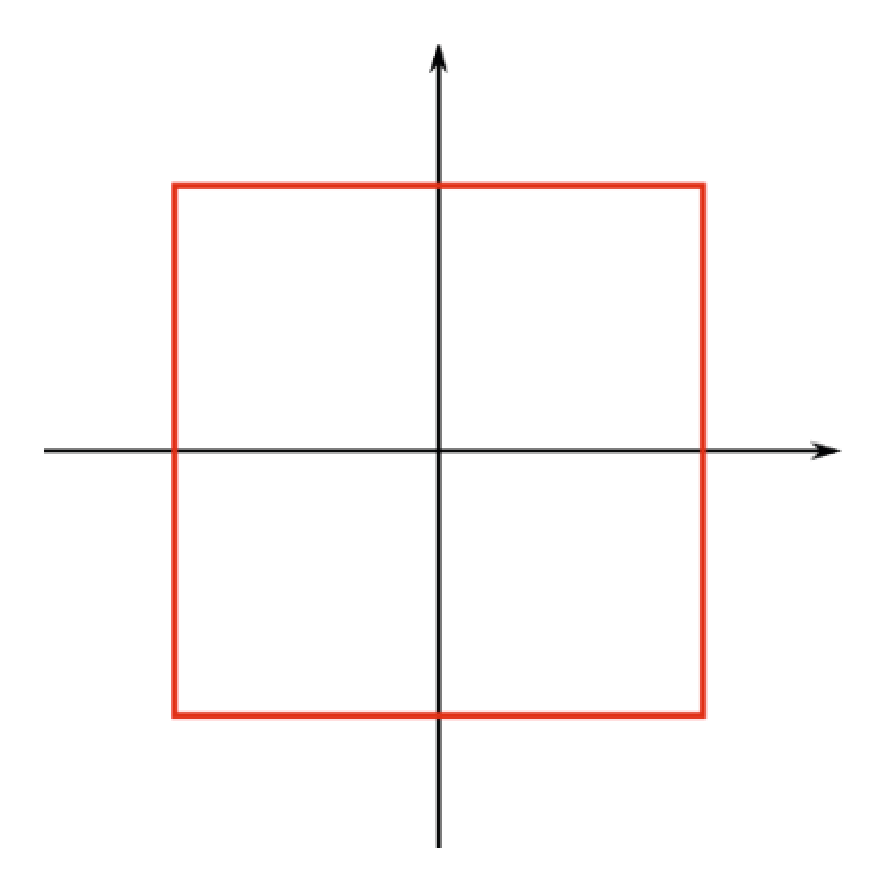
\includegraphics[scale=0.35]{fig3_1} 
		\figcaption{正方形}
	}
	
	\marginpar{
		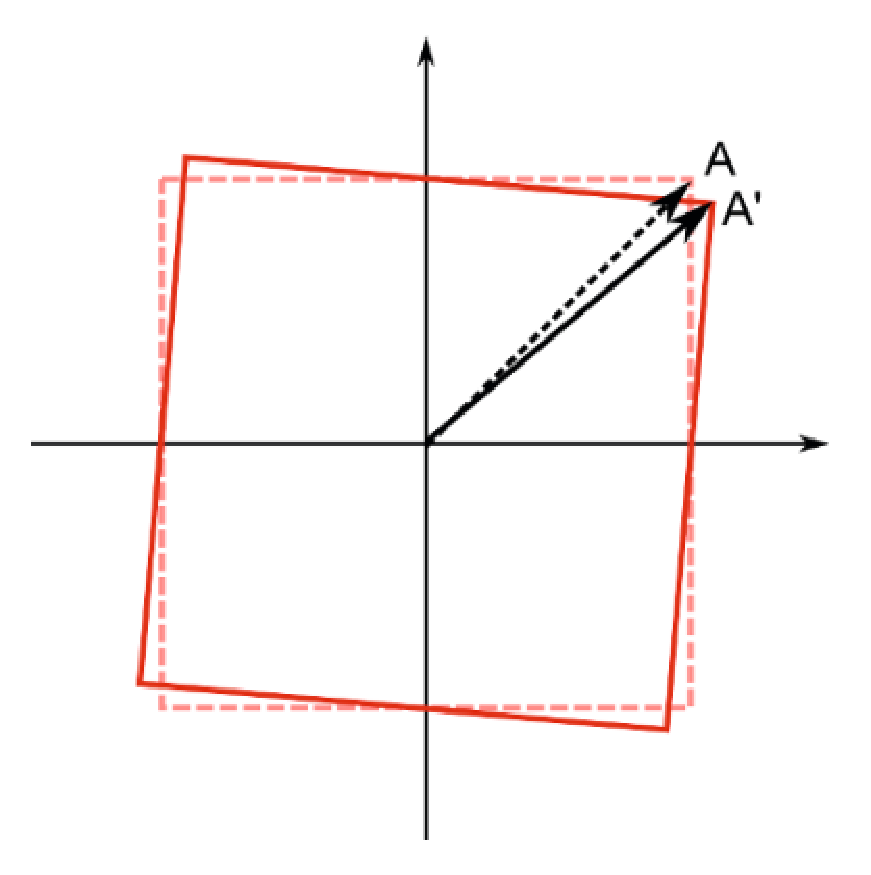
\includegraphics[scale=0.35]{fig3_2.eps}
		\figcaption{正方形绕中心顺时针旋转$5^\circ$}
	}
	
	注意不是所有旋转变换都对称. 我们关注顶点的变化就能看出来, 比如绕中心顺时针旋转$5^\circ$, 这个变换将顶点映射到原来正方形点集之外, 顶点$A$映射到了原来正方形集合之外的点$A'$. 因此这个旋转变换对正方形不具有对称性. 当然, 变换后的点集仍然是个正方形, 但却是不同的正方形(即不同点的集合). 绕中心转$90^\circ$是对称的, 如图\ref{fig3.3}, 顶点$A$变换到点$B$, 等等, 原来的正方形点集变换到相同的集合.
	
	{
	\centering{
	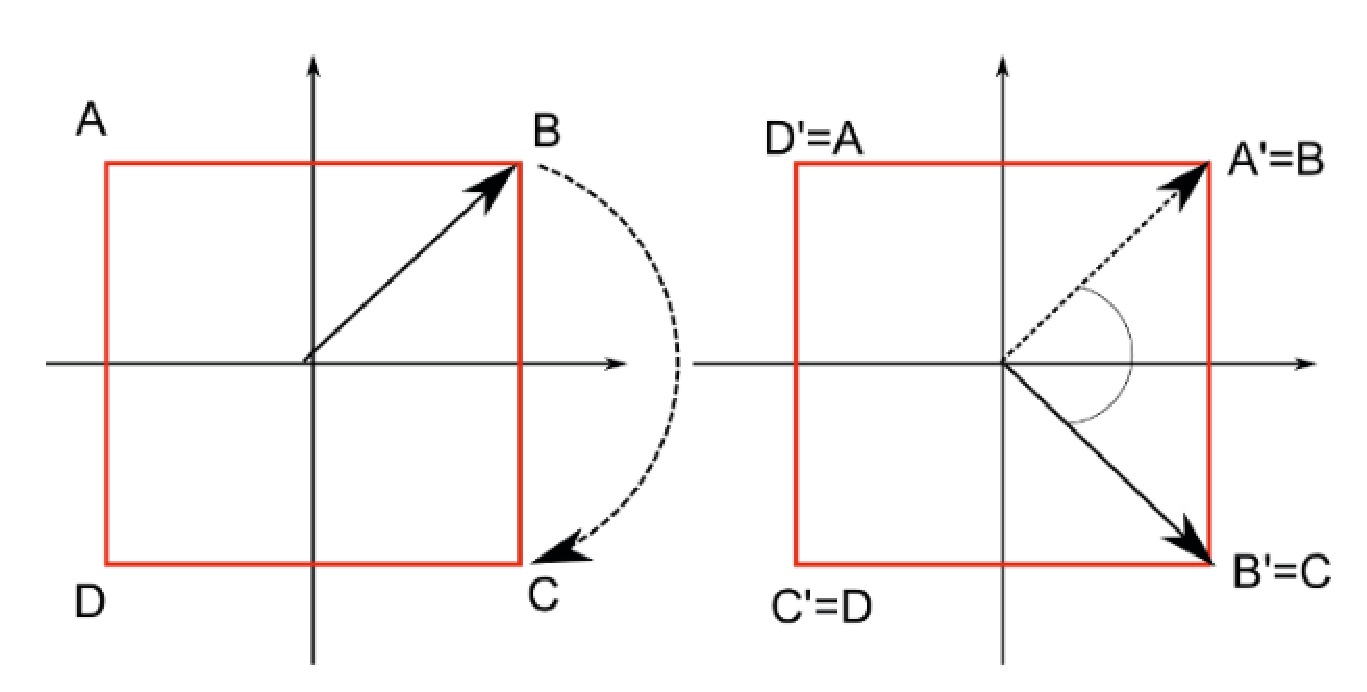
\includegraphics[scale=0.4]{fig3_3}
	\figcaption{正方形绕中心旋转$90^\circ$}
	\label{fig3.3}
	}}
	
	假如你看了一眼原来的正方形, 然后闭上眼睛, 这时有人把正方形做了一个变换. 如果你不能分辨这个正方形是否发生变化, 那么这个变换就是个对称变换.
	
	我们把所有使正方形不变的变换构成的集合称为群. 变换参数(本例中就是旋转角度)不能任意取值(而是取分立的数), 这个群称为离散群.
	
	\item 另一个例子是使单位圆不变的变换构成的集合. 类似地, 单位圆还是一些点构成的集合, 对称变换把这个集合映射到它自身.
	
	单位圆绕圆心旋转任意角度都不变. 换言之, 变换参数(这里就是旋转角度)可以取任意值, 因此这个群称为连续群.
\end{enumerate}
	\marginpar{
		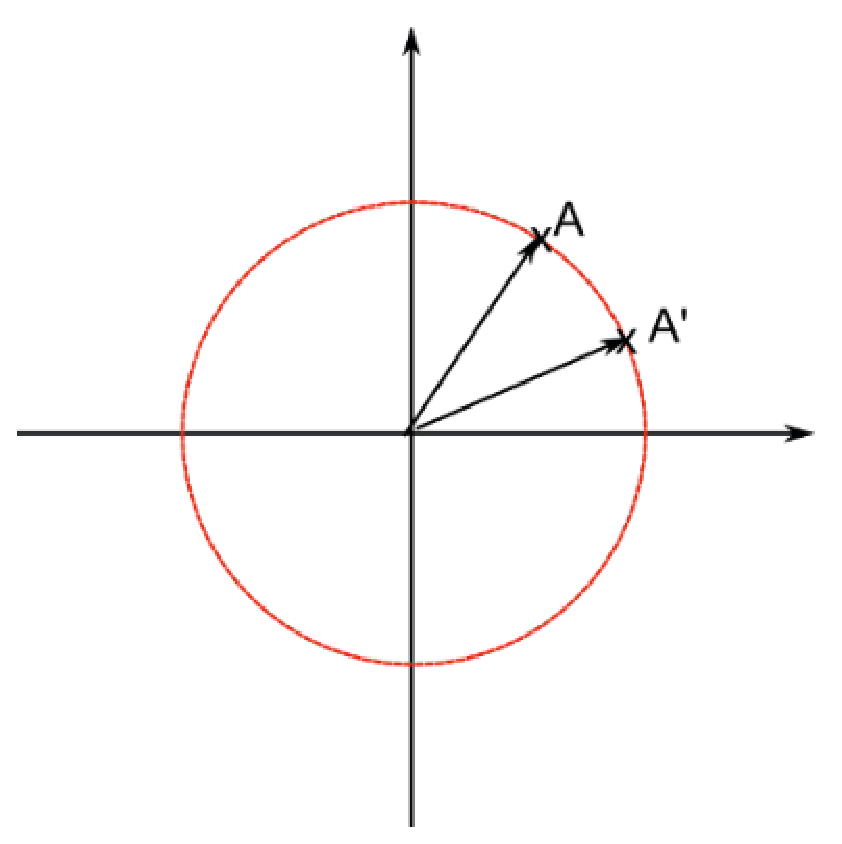
\includegraphics[scale=0.35]{fig3_4.eps}
		\figcaption{单位圆绕圆心旋转任意角度都不变}
	}

数学中除了几何图形之外还有好多别的都有对称性. 例如,对于向量, 我们可以考虑所有让向量长度不变的变换构成的集合. 看出本节开头对称性定义的普遍性了没? 对称性就是变换下的不变性. 非常幸运, 搞数学的早已建立了群论, 它可以研究所有类型的对称性\mpar{历史上数学家们建立群论最初是为了描述方程的对称性}.

为了让精确描述对称性的工具 --- 群的定义来的自然一点, 我们把对称性的定义用数学语言精炼一下:
\begin{itemize}
	\item 对某物什么也不做(比如转个$0^\circ$)当然也是对称变换(按照我们的对称性定义), 因此任何群都需要包含一个恒等变换(恒等元). 在上面的例子里, 恒等元就是旋转$0^\circ$.
	
	\item 对某物先做变换再做逆变换的结果必须等于啥也不做. 因此对于群中的任意元素(简称群元), 必须有相应的逆元素. 按定义, 先做变换再做逆变换等于恒等变换. 例如先转$90^\circ$再转$-90^\circ$(先逆针再顺针转)与旋转$0^\circ$相同.
	
	\item 先做一个对称变换再做一个对称变换, 总体效果必须还是对称变换. 例如先旋转$90^\circ$再转$180^\circ$等于直接转$270^\circ$, 后者也是对称变换. 对称变换的这个性质称为封闭性.
	
	\item 对称变换之间必须满足结合律. 例如先转$90^\circ$再转$40^\circ$再转$110^\circ$与先转$130^\circ$再转$110^\circ$相同, 先转$90^\circ$再转$150^\circ$也一样. 用符号表示更加清楚:
	\begin{equation}\label{equ3.1}
	R(110^\circ) R(40^\circ) R(90^\circ) = R(110^\circ)\bigg( R(40^\circ)R(90^\circ) \bigg) = R(110^\circ) R(130^\circ)
	\end{equation}
	\begin{equation}\label{equ3.2}
	R(110^\circ) R(40^\circ) R(90^\circ) = \bigg( R(110^\circ) R(40^\circ) \bigg) R(90^\circ) = R(150^\circ) R(90^\circ)
	\end{equation}
	这个性质称为{\bf 结合律}.
	
	\item 我们要有规定两个群元(对称变换)怎样合体的规则, 它是个{\bf 二元运算}(两个群元合体成一个), 我们称它为{\bf 群乘法}. 
	
	在上面的例子里, 旋转变换的标准表示方法是用旋转矩阵\mpar{旋转矩阵见附录A.2.}, 两个群元(两个旋转矩阵, 或两个旋转操作)合体的规则是线性代数里的矩阵乘法. 同样的变换经常有不同的表示方法\mpar{例如, 二维平面旋转还可以用单位复数描述, 相应的群乘法是复数乘法. 稍后就讨论这一点.}, 群论非常系统性地概括了所有形式. 群论的分支 --- {\bf 表示论}就是研究相同变换的不同描述方式的, 我们在\ref{sec3.5}节学习表示论.
\end{itemize}

\ 

我们把上述群与对称变换的特征用严谨的数学语言表达, 再将它们提升为公理, 满足这些公理的数学结构就是一个群. 数学系的群论书可能更喜欢在开头就从天上掉下来这些公理. 必须指出满足群公理的结构可能是超级抽象的, 但我们现在只关注上面例子里的旋转变换那样的群. \sout{因为我们是物理系的, 而且这是本物理书}

\ 

(我们通过对称变换的性质导出的)群公理\mpar{别担心怎么才能根据这些公理凑出一个群来. 搞物理的往往是从某个变换出发, 考察它是否符合群公理, 如果是\sout{经常是}那么就可以应用群论来解决问题.}: 

一个群就是一个集合$G$加上一个定义在$G$上的二元运算(群乘法)$\circ$, 当然$(G, \circ)$还要满足以下公理: 
\begin{itemize}
	\item 封闭性: 对于任意$g_1, g_2 \in G, g_1 \circ g_2 \in G$
	
	\item 单位元: 存在单位元$e \in G$使得对于所有$g \in G, g\circ e = g = e \circ g$
	
	\item 逆元: 对于任意$g \in G$, 存在相应的逆元$g^{-1} \in G$使得$g \circ g^{-1} = e = g^{-1} \circ g$
	
	\item 结合律: 对于任意$g_1, g_2, g_3 \in G, g_1 \circ (g_2 \circ g_3) = (g_1 \circ g_2) \circ g_3$ 
\end{itemize}

总结: 某物体在一些变换下保持不变, 这些变换组成\footnote{我在想这里该用`构成'还是`组成', 后来我觉得无所谓, 因为这不是初中化学...(分子构成物质, 元素组成物质...) --- 译者(SI)}的集合叫做对称群. 对于Minkowski时空, Minkowski度规\mpar{复习一下, Minkowski度规就是在Minkowski空间中用来计算距离和长度的工具, 见第二章.}在变换下保持不变, 相应的对称群称为Poincare群.

要注意群的定义完全与变换的物体是啥没有关系. 我们可以脱离特定物体而只研究对称变换本身, 群的定义将变换从物体中`提取'出来了. 这是非常有用的, 许多不同事物具有同样或同类的对称性. 群论让我们不用管变换的物体(圆还是正方形), 只研究变换(例如旋转)的普遍性质.







%!TEX encoding = UTF-8 Unicode

%----------------------------------------------------------------------------------------
%	CHAPTER 4
%----------------------------------------------------------------------------------------

\chapterimage{chapter_head_1.pdf} % Chapter heading image

\chapter{The Framework 框架/参考系}
这一章的基本思路是,我们要在尽可能少的使用\emph{某些东西}的前提下,得到正确的关于自然的方程。\emph{某些东西}是什么?有一件事是确定的:它不应该在 Lorentz 变换下改变,否则我们会在不同的参考系下得到不同的自然规律。在数学意义上,这意味着我们寻找的这个东西是个标量,依照洛伦兹群的 \( (0,0) \) 表示作变换。考虑到自然总依简单而行,这足以让我们导出关于自然的方程了。

%flag The equations of nature



%\begin{table}[h]
%\centering
%\begin{tabular}{l l l}
%\toprule
%\textbf{Treatments} & \textbf{Response 1} & \textbf{Response 2}\\
%\midrule
%Treatment 1 & 0.0003262 & 0.562 \\
%Treatment 2 & 0.0015681 & 0.910 \\
%Treatment 3 & 0.0009271 & 0.296 \\
%\bottomrule
%\end{tabular}
%\caption{Table caption}
%\end{table}

%\chapter*{Bibliography}
%\addcontentsline{toc}{chapter}{\textcolor{ocre}{Bibliography}}
%\section*{Books}
%\addcontentsline{toc}{section}{Books}
%\printbibliography[heading=bibempty,type=book]
%\section*{Articles}
%\addcontentsline{toc}{section}{Articles}
%\printbibliography[heading=bibempty,type=article]

%----------------------------------------------------------------------------------------
%	INDEX
%----------------------------------------------------------------------------------------

%\cleardoublepage
%\phantomsection
%\setlength{\columnsep}{0.75cm}
%\addcontentsline{toc}{chapter}{\textcolor{ocre}{Index}}
%\printindex

%----------------------------------------------------------------------------------------
%\cleardoublepage
%\bibliographystyle{apsrev4-1}
%\bibliography{bibliography}
\end{spacing}



\end{document}